% Options for packages loaded elsewhere
\PassOptionsToPackage{unicode}{hyperref}
\PassOptionsToPackage{hyphens}{url}
%
\documentclass[
  oneside]{book}
\usepackage{amsmath,amssymb}
\usepackage{lmodern}
\usepackage{iftex}
\ifPDFTeX
  \usepackage[T1]{fontenc}
  \usepackage[utf8]{inputenc}
  \usepackage{textcomp} % provide euro and other symbols
\else % if luatex or xetex
  \usepackage{unicode-math}
  \defaultfontfeatures{Scale=MatchLowercase}
  \defaultfontfeatures[\rmfamily]{Ligatures=TeX,Scale=1}
\fi
% Use upquote if available, for straight quotes in verbatim environments
\IfFileExists{upquote.sty}{\usepackage{upquote}}{}
\IfFileExists{microtype.sty}{% use microtype if available
  \usepackage[]{microtype}
  \UseMicrotypeSet[protrusion]{basicmath} % disable protrusion for tt fonts
}{}
\makeatletter
\@ifundefined{KOMAClassName}{% if non-KOMA class
  \IfFileExists{parskip.sty}{%
    \usepackage{parskip}
  }{% else
    \setlength{\parindent}{0pt}
    \setlength{\parskip}{6pt plus 2pt minus 1pt}}
}{% if KOMA class
  \KOMAoptions{parskip=half}}
\makeatother
\usepackage{xcolor}
\IfFileExists{xurl.sty}{\usepackage{xurl}}{} % add URL line breaks if available
\IfFileExists{bookmark.sty}{\usepackage{bookmark}}{\usepackage{hyperref}}
\hypersetup{
  pdftitle={Booklet for the PiER},
  hidelinks,
  pdfcreator={LaTeX via pandoc}}
\urlstyle{same} % disable monospaced font for URLs
\usepackage{longtable,booktabs,array}
\usepackage{calc} % for calculating minipage widths
% Correct order of tables after \paragraph or \subparagraph
\usepackage{etoolbox}
\makeatletter
\patchcmd\longtable{\par}{\if@noskipsec\mbox{}\fi\par}{}{}
\makeatother
% Allow footnotes in longtable head/foot
\IfFileExists{footnotehyper.sty}{\usepackage{footnotehyper}}{\usepackage{footnote}}
\makesavenoteenv{longtable}
\usepackage{graphicx}
\makeatletter
\def\maxwidth{\ifdim\Gin@nat@width>\linewidth\linewidth\else\Gin@nat@width\fi}
\def\maxheight{\ifdim\Gin@nat@height>\textheight\textheight\else\Gin@nat@height\fi}
\makeatother
% Scale images if necessary, so that they will not overflow the page
% margins by default, and it is still possible to overwrite the defaults
% using explicit options in \includegraphics[width, height, ...]{}
\setkeys{Gin}{width=\maxwidth,height=\maxheight,keepaspectratio}
% Set default figure placement to htbp
\makeatletter
\def\fps@figure{htbp}
\makeatother
\setlength{\emergencystretch}{3em} % prevent overfull lines
\providecommand{\tightlist}{%
  \setlength{\itemsep}{0pt}\setlength{\parskip}{0pt}}
\setcounter{secnumdepth}{5}
\ifLuaTeX
  \usepackage{selnolig}  % disable illegal ligatures
\fi

\title{Booklet for the PiER}
\author{}
\date{\vspace{-2.5em}}

\begin{document}
\maketitle

{
\setcounter{tocdepth}{2}
\tableofcontents
}
\hypertarget{index}{%
\chapter{Background}\label{index}}

\begin{figure}

{\centering 
\includegraphics[width=0.3\linewidth]{index_files/figure-latex/logo-1} 

}

\caption{The logo for the web-based facilities - PiER that enables and automates genetics-led and network-based genetic target prioritisation.}\label{fig:logo}
\end{figure}

\begin{quote}
\textbf{Motivation}
\end{quote}

We and others are leading the field of target discovery through developing approaches for genetics-led target prioritisation. Integrative prioritisation for early-stage genetic target discovery has been demonstrated to be cost-effective in promoting the translational use of disease genetic associations, a principle increasingly recognised to reduce drug attrition rate in late-stage clinical trials.

\begin{quote}
\textbf{Design}
\end{quote}

Building on our well-established algorithm (see \href{https://www.ncbi.nlm.nih.gov/pubmed/31253980}{Nature Genetics 2019}), here I introduce web-based servers/facilities called \texttt{PiER}. The PiER is free and open to all users and there is no login requirement, allowing the users to perform real-time target prioritisation harnessing human disease genetics, functional genomics, and protein interactions.

By analogy to the piano \href{https://www.piano-keyboard-guide.com/grand-staff.html}{stave}, the PiER consists of five horizontal lines, with three lines representing the elementary facility (\texttt{eV2CG}, \texttt{eCG2PG} and \texttt{eCrosstalk}), each doing specific tasks on their own, and the rest two lines signifying the combinatory facility (\texttt{cTGene} and \texttt{cTCrosstalk}), making the prioritisaton process transparent to follow and easy to use.

\begin{itemize}
\item
  \protect\hyperlink{ev2cg}{eV2CG}, linking variants to core genes; see \href{http://www.genetictargets.com/app/examples/_tmp_RMD_eV2CG.html}{Sample Output}
\item
  \protect\hyperlink{ecg2pg}{eCG2PG}, networking core genes to peripheral genes; see \href{http://www.genetictargets.com/app/examples/_tmp_RMD_eCG2PG.html}{Sample Output}
\item
  \protect\hyperlink{ecrosstalk}{eCrosstalk}, identifying the crosstalk between pathways; see \href{http://www.genetictargets.com/app/examples/_tmp_RMD_eCrosstalk.html}{Sample Output}
\item
  \protect\hyperlink{ctgene}{cTGene}, prioritising targets at the gene level; see \href{http://www.genetictargets.com/app/examples/_tmp_RMD_cTGene.html}{Sample Output}
\item
  \protect\hyperlink{ctcrosstalk}{cTCrosstalk}, prioritising targets at the crosstalk level; see \href{http://www.genetictargets.com/app/examples/_tmp_RMD_cTCrosstalk.html}{Sample Output}
\end{itemize}

\hypertarget{facilities}{%
\chapter{Facilities}\label{facilities}}

The elementary facility supports three specific tasks, including: (i) \texttt{eV2CG}, utilising functional genomics to link disease-associated variants (including those located at the non-coding genome) to core genes likely responsible for genetic associations; (ii) \texttt{eCG2PG}, using knowledge of protein interactions to `network' core genes to each other and also to additional peripheral genes, producing a ranked list of core and peripheral genes; and (iii) \texttt{eCrosstalk}, exploiting the information of pathway-derived interactions to identify highly ranked genes that mediate the crosstalk between molecular pathways. Through chaining together elementary tasks supported in the elementary facility, the combinatory facility enables the automation of genetics-led and network-based integrative prioritisation for genetic targets at the gene level (\texttt{cTGene}) and also at the crosstalk level (\texttt{cTCrosstalk}). Notably, in addition to target crosstalk, the \texttt{cTCrosstalk} further supports target pathway prioritisation and crosstalk-based drug repurposing analysis (that is, repositioning approved drugs into new disease indications).

\begin{figure}

{\centering 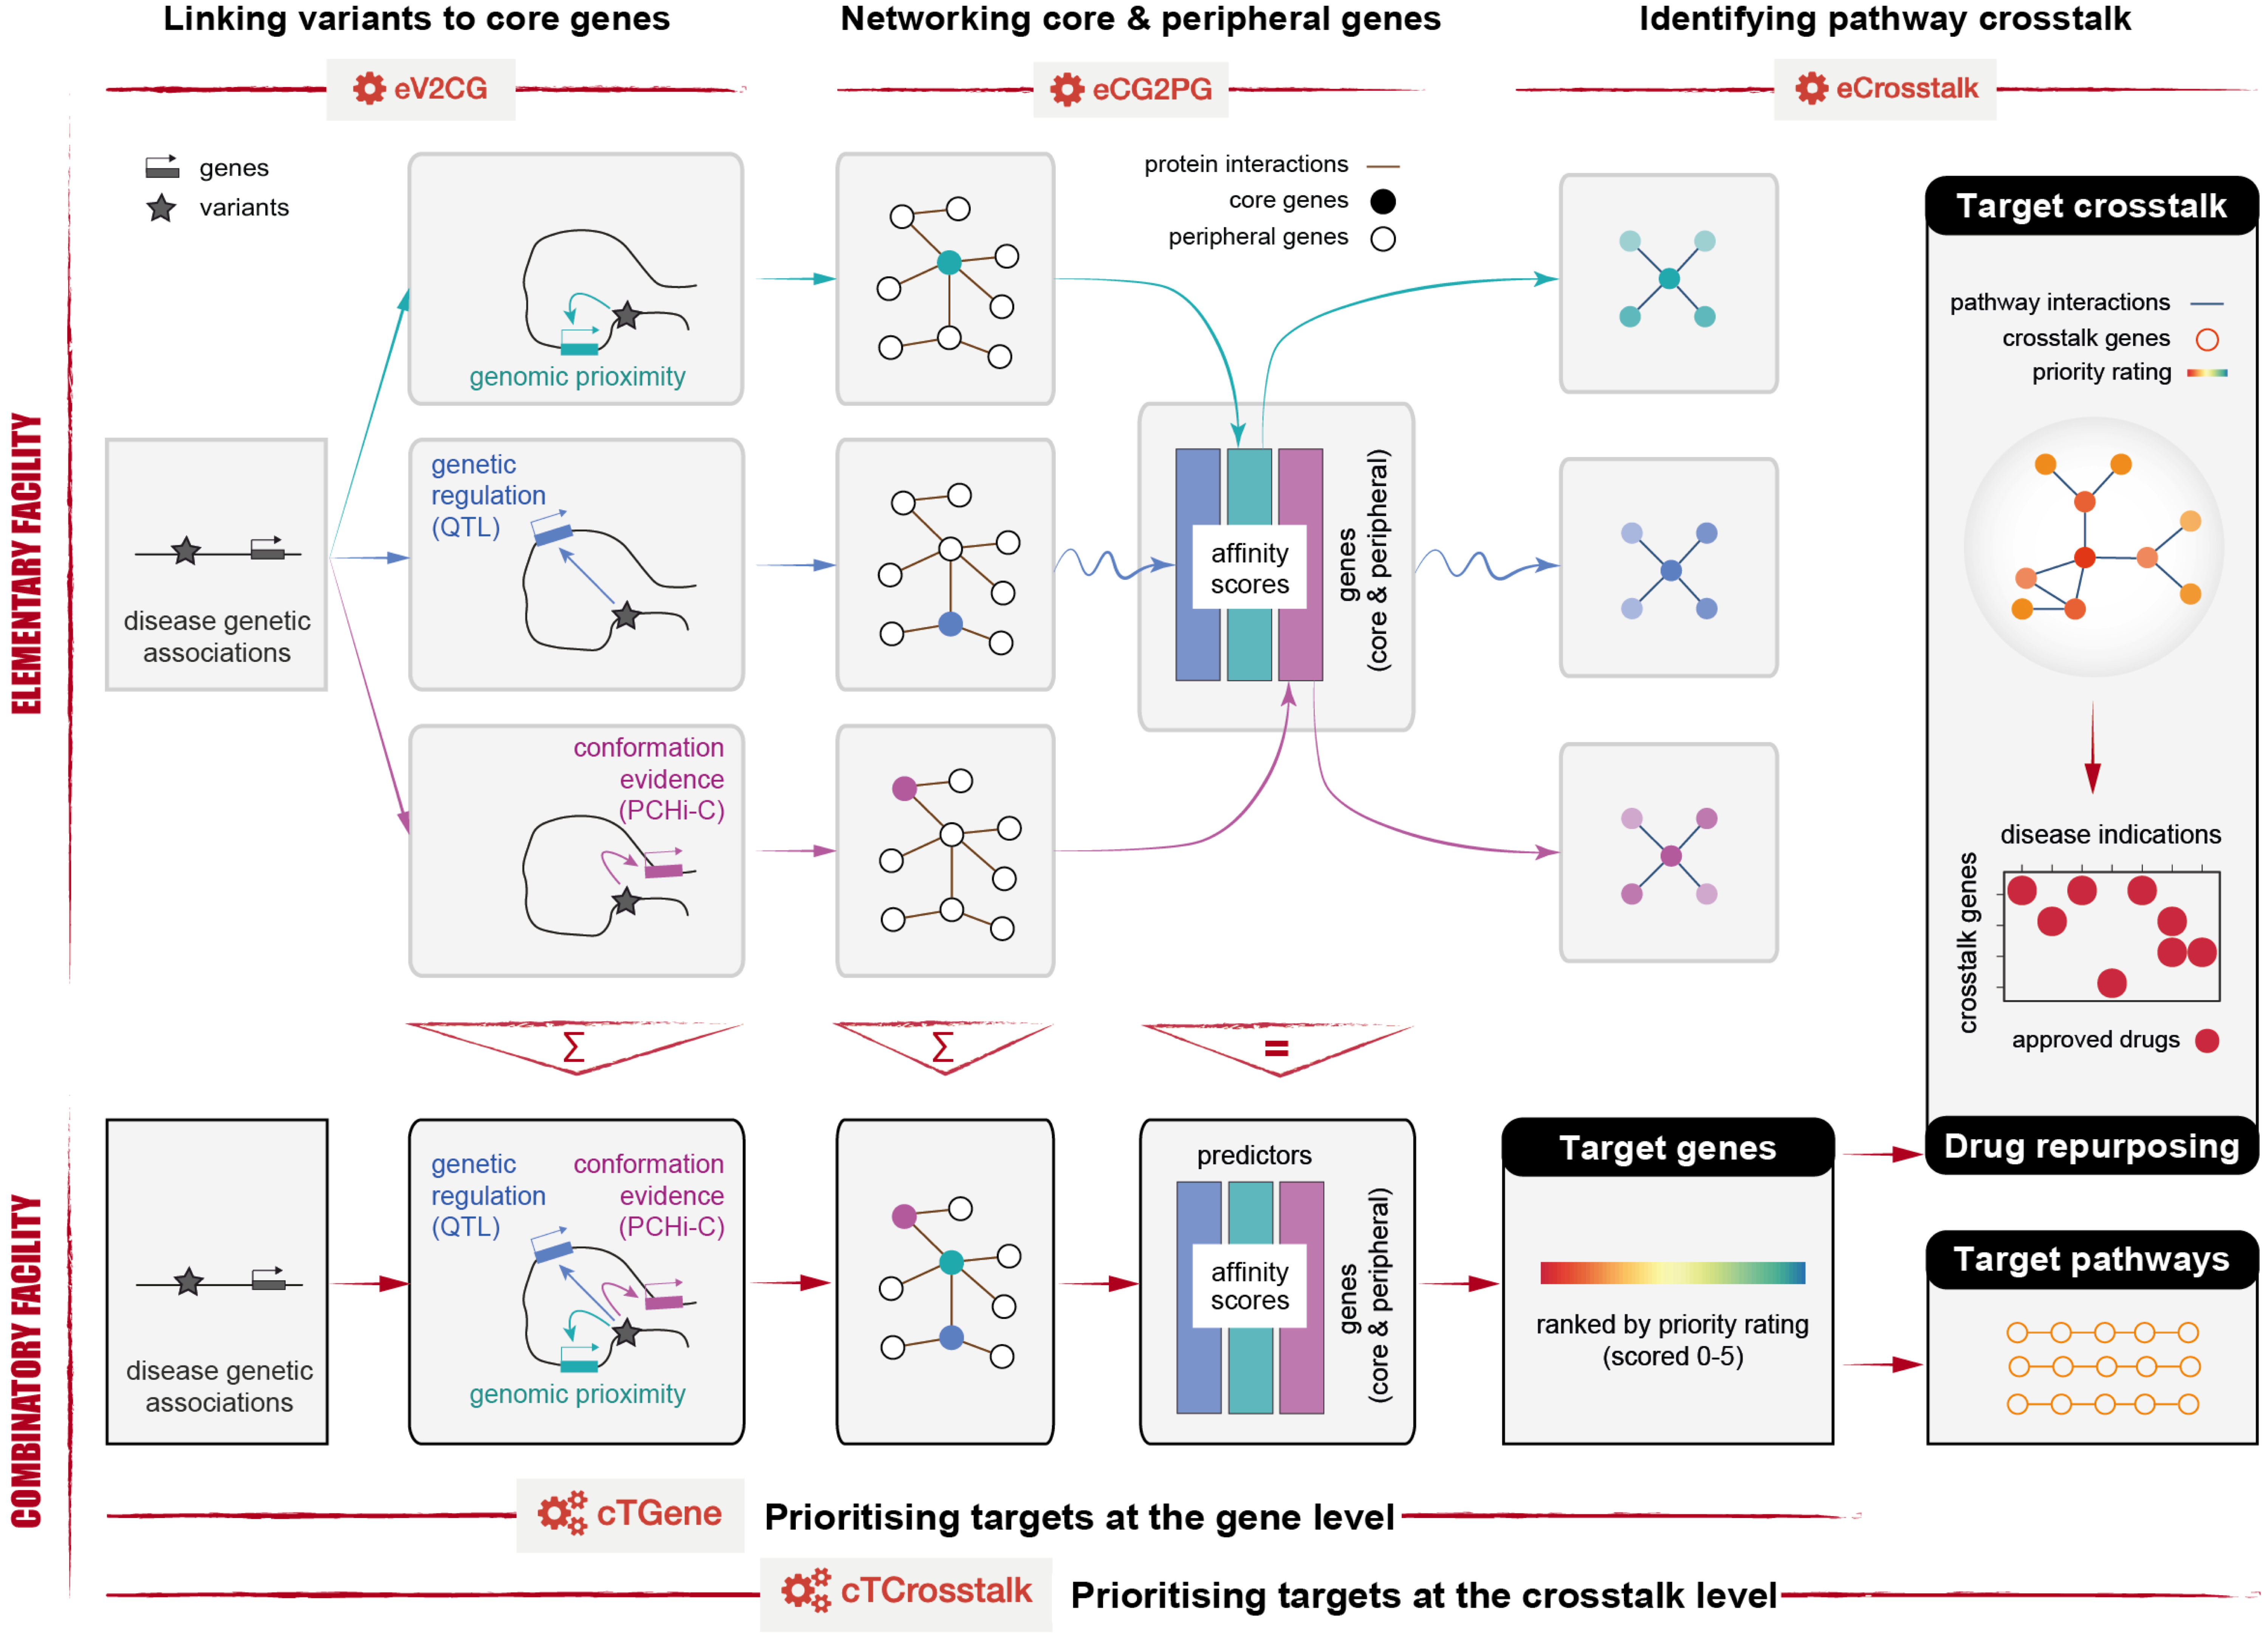
\includegraphics[width=1\linewidth]{index_files/figure-latex/design-1} 

}

\caption{Schematic illustration of two facilities supported in the PiER.}\label{fig:design}
\end{figure}

\hypertarget{compatibility}{%
\chapter{Compatibility}\label{compatibility}}

\begin{table}

\caption{\label{tab:unnamed-chunk-3}A summary of the PiER website browser compatibility.}
\centering
\begin{tabular}[t]{l|c|c|c}
\hline
  & MacOS (Big Sur) & Windows (10) & Linux (Ubuntu)\\
\hline
Safari & 14.1.2 & N/A & N/A\\
\hline
Microsoft Edge & N/A & 85.0.564.67 & N/A\\
\hline
Google Chrome & 96.0.4664.110 & 90.0.4430.93 & 96.0.4664.110\\
\hline
Firefox & 95.0.2 & 95.0.2 & 95.0.2\\
\hline
\end{tabular}
\end{table}

\hypertarget{runtime}{%
\chapter{Runtime}\label{runtime}}

\begin{table}

\caption{\label{tab:unnamed-chunk-4}A summary of the estimated runtime.}
\centering
\begin{tabular}[t]{c|c|c}
\hline
Facilities & Tools & Runtime (Server + Client)\\
\hline
Elementary & eV2CG & (67 + 82) seconds\\
\hline
Elementary & eCG2PG & (15 + 70) seconds\\
\hline
Elementary & eCrosstalk & (53 + 71) seconds\\
\hline
Combinatory & cTGene & (90 + 91) seconds\\
\hline
Combinatory & cTCrosstalk & (143 + 97) seconds\\
\hline
\end{tabular}
\end{table}

\hypertarget{frontpage}{%
\chapter{Frontpage}\label{frontpage}}

\begin{figure}

{\centering 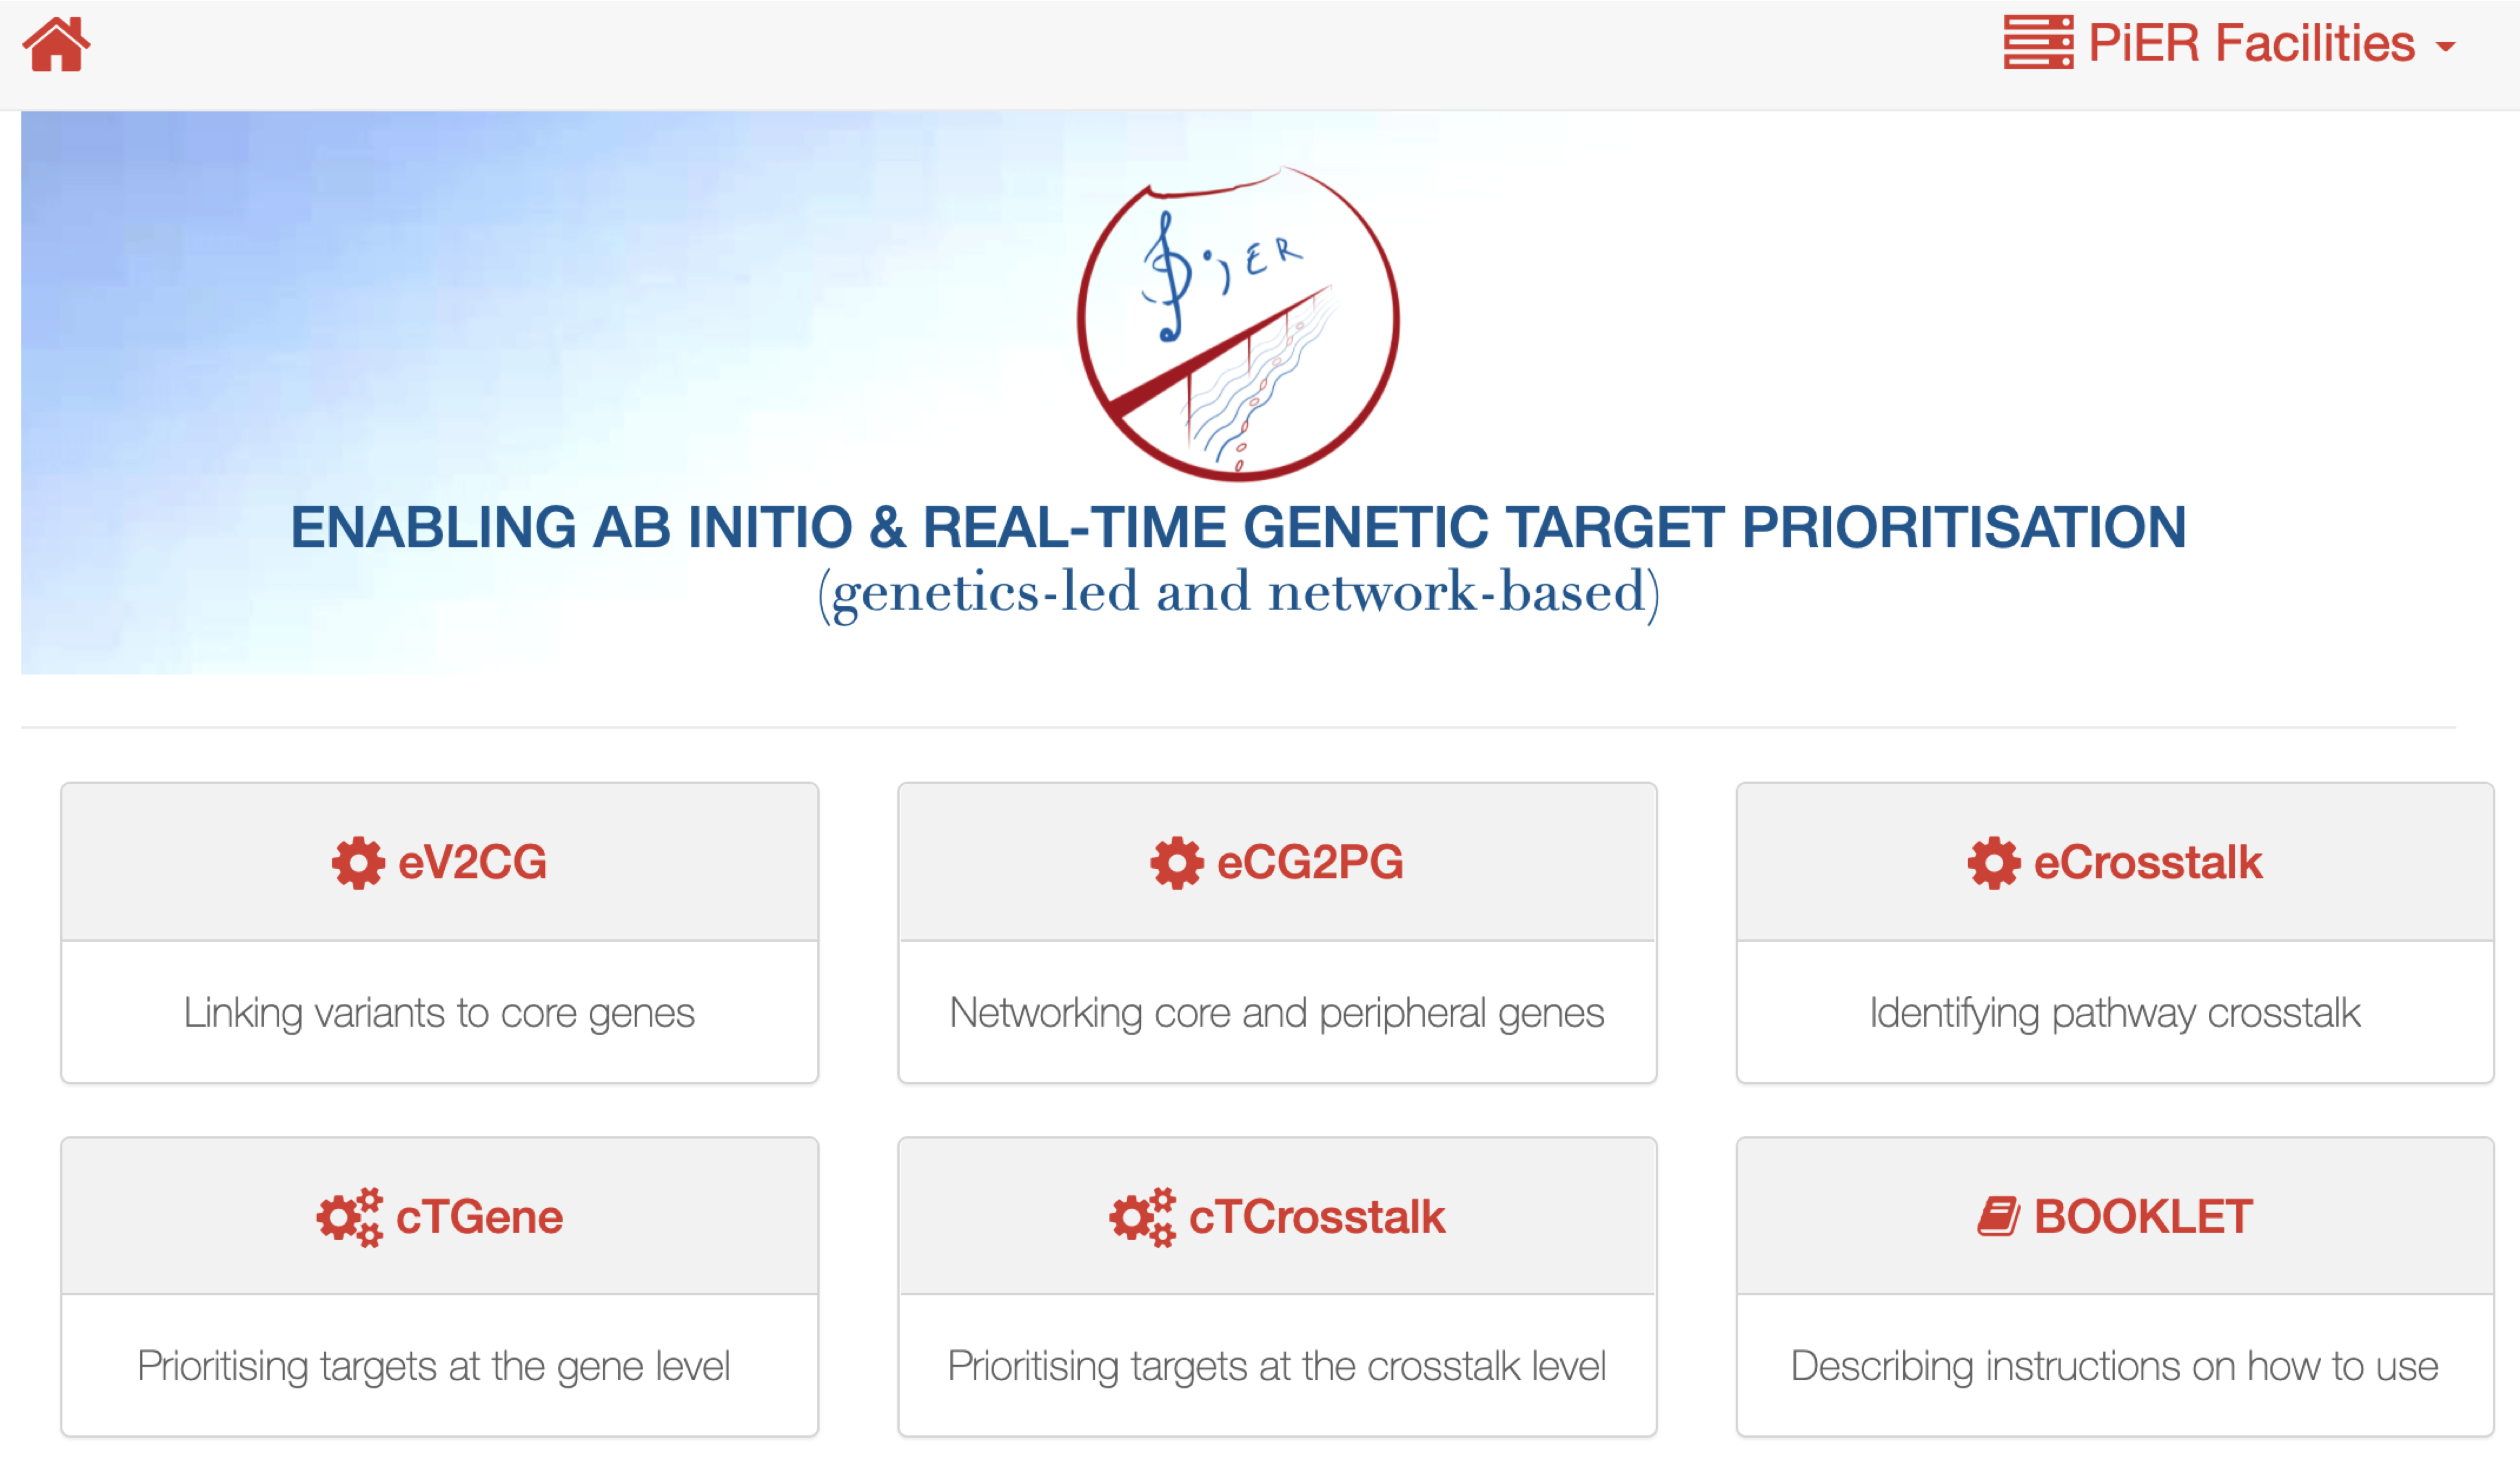
\includegraphics[width=1\linewidth]{index_files/figure-latex/app-front-1} 

}

\caption{The landing frontpage of the PiER, featuring two facilities (elementary and combinatory). The elementary facility includes: (i) eV2CG, linking disease associated variants (particularly located at the non-coding genomic region) to (core) genes likely responsible for associations, based on either conformation evidence (that is, promoter-centered chromatin interactions), quantitative trait locus (QTL) mapping (that is, genetic regulation of gene expression or protein abundance), or simply genomic proximity; (ii) eCG2PG, using the knowledge of protein interactions to ‘network’ core genes to each other and to additional (peripheral) genes as well, generating a ranked list of core and peripheral genes; and (iii) eCrosstalk, exploiting the information of well-curated pathway-derived interactions to identify the subnetwork of highly ranked genes that mediate pathway crosstalk. Chaining together elementary functionalities above into pipelines provides the combinatory facility, enabling/automating genetics-led and network-based identification and prioritisation of drug targets: (iv) at the gene level (cTGene); and (v) at the crosstalk level (cTCrosstalk). Also included is the tutorial-like booklet (in a HTML- and PDF-format) of explaining step-by-step instructions.}\label{fig:app-front}
\end{figure}

\hypertarget{ev2cg}{%
\chapter{eV2CG}\label{ev2cg}}

\hypertarget{interface}{%
\section{Interface}\label{interface}}

\begin{quote}
\textbf{Input}
\end{quote}

\begin{itemize}
\tightlist
\item
  \texttt{Step\ 1}: a list of user-defined SNPs (1st column for dbSNP rsIDs, 2nd for significance info). By default, sample data are shared genetic variants identified from cross-disease genome-wide association studies in inflammatory disorders; see \href{https://www.ncbi.nlm.nih.gov/pubmed/26974007}{Nature Genetics 2016}.
\end{itemize}

\begin{quote}
\textbf{Mechanism}
\end{quote}

\begin{itemize}
\item
  \texttt{Step\ 2}: includes SNPs in Linkage Disequilibrium (LD).
\item
  \texttt{Step\ 3}: uses genomic proximity, quantitative trait locus (QTL), or promoter capture Hi-C data to identify core genes.
\item
  \texttt{More\ controls}: fine-tunes parameters involved in steps described above.
\end{itemize}

\begin{quote}
\textbf{Output}
\end{quote}

\begin{itemize}
\tightlist
\item
  \href{http://www.genetictargets.com/app/examples/_tmp_RMD_eV2CG.html}{Sample Output} includes an interactive table for core genes, and a manhattan plot (illustrating scored core genes color-coded by chromosomes).
\end{itemize}

\begin{figure}

{\centering 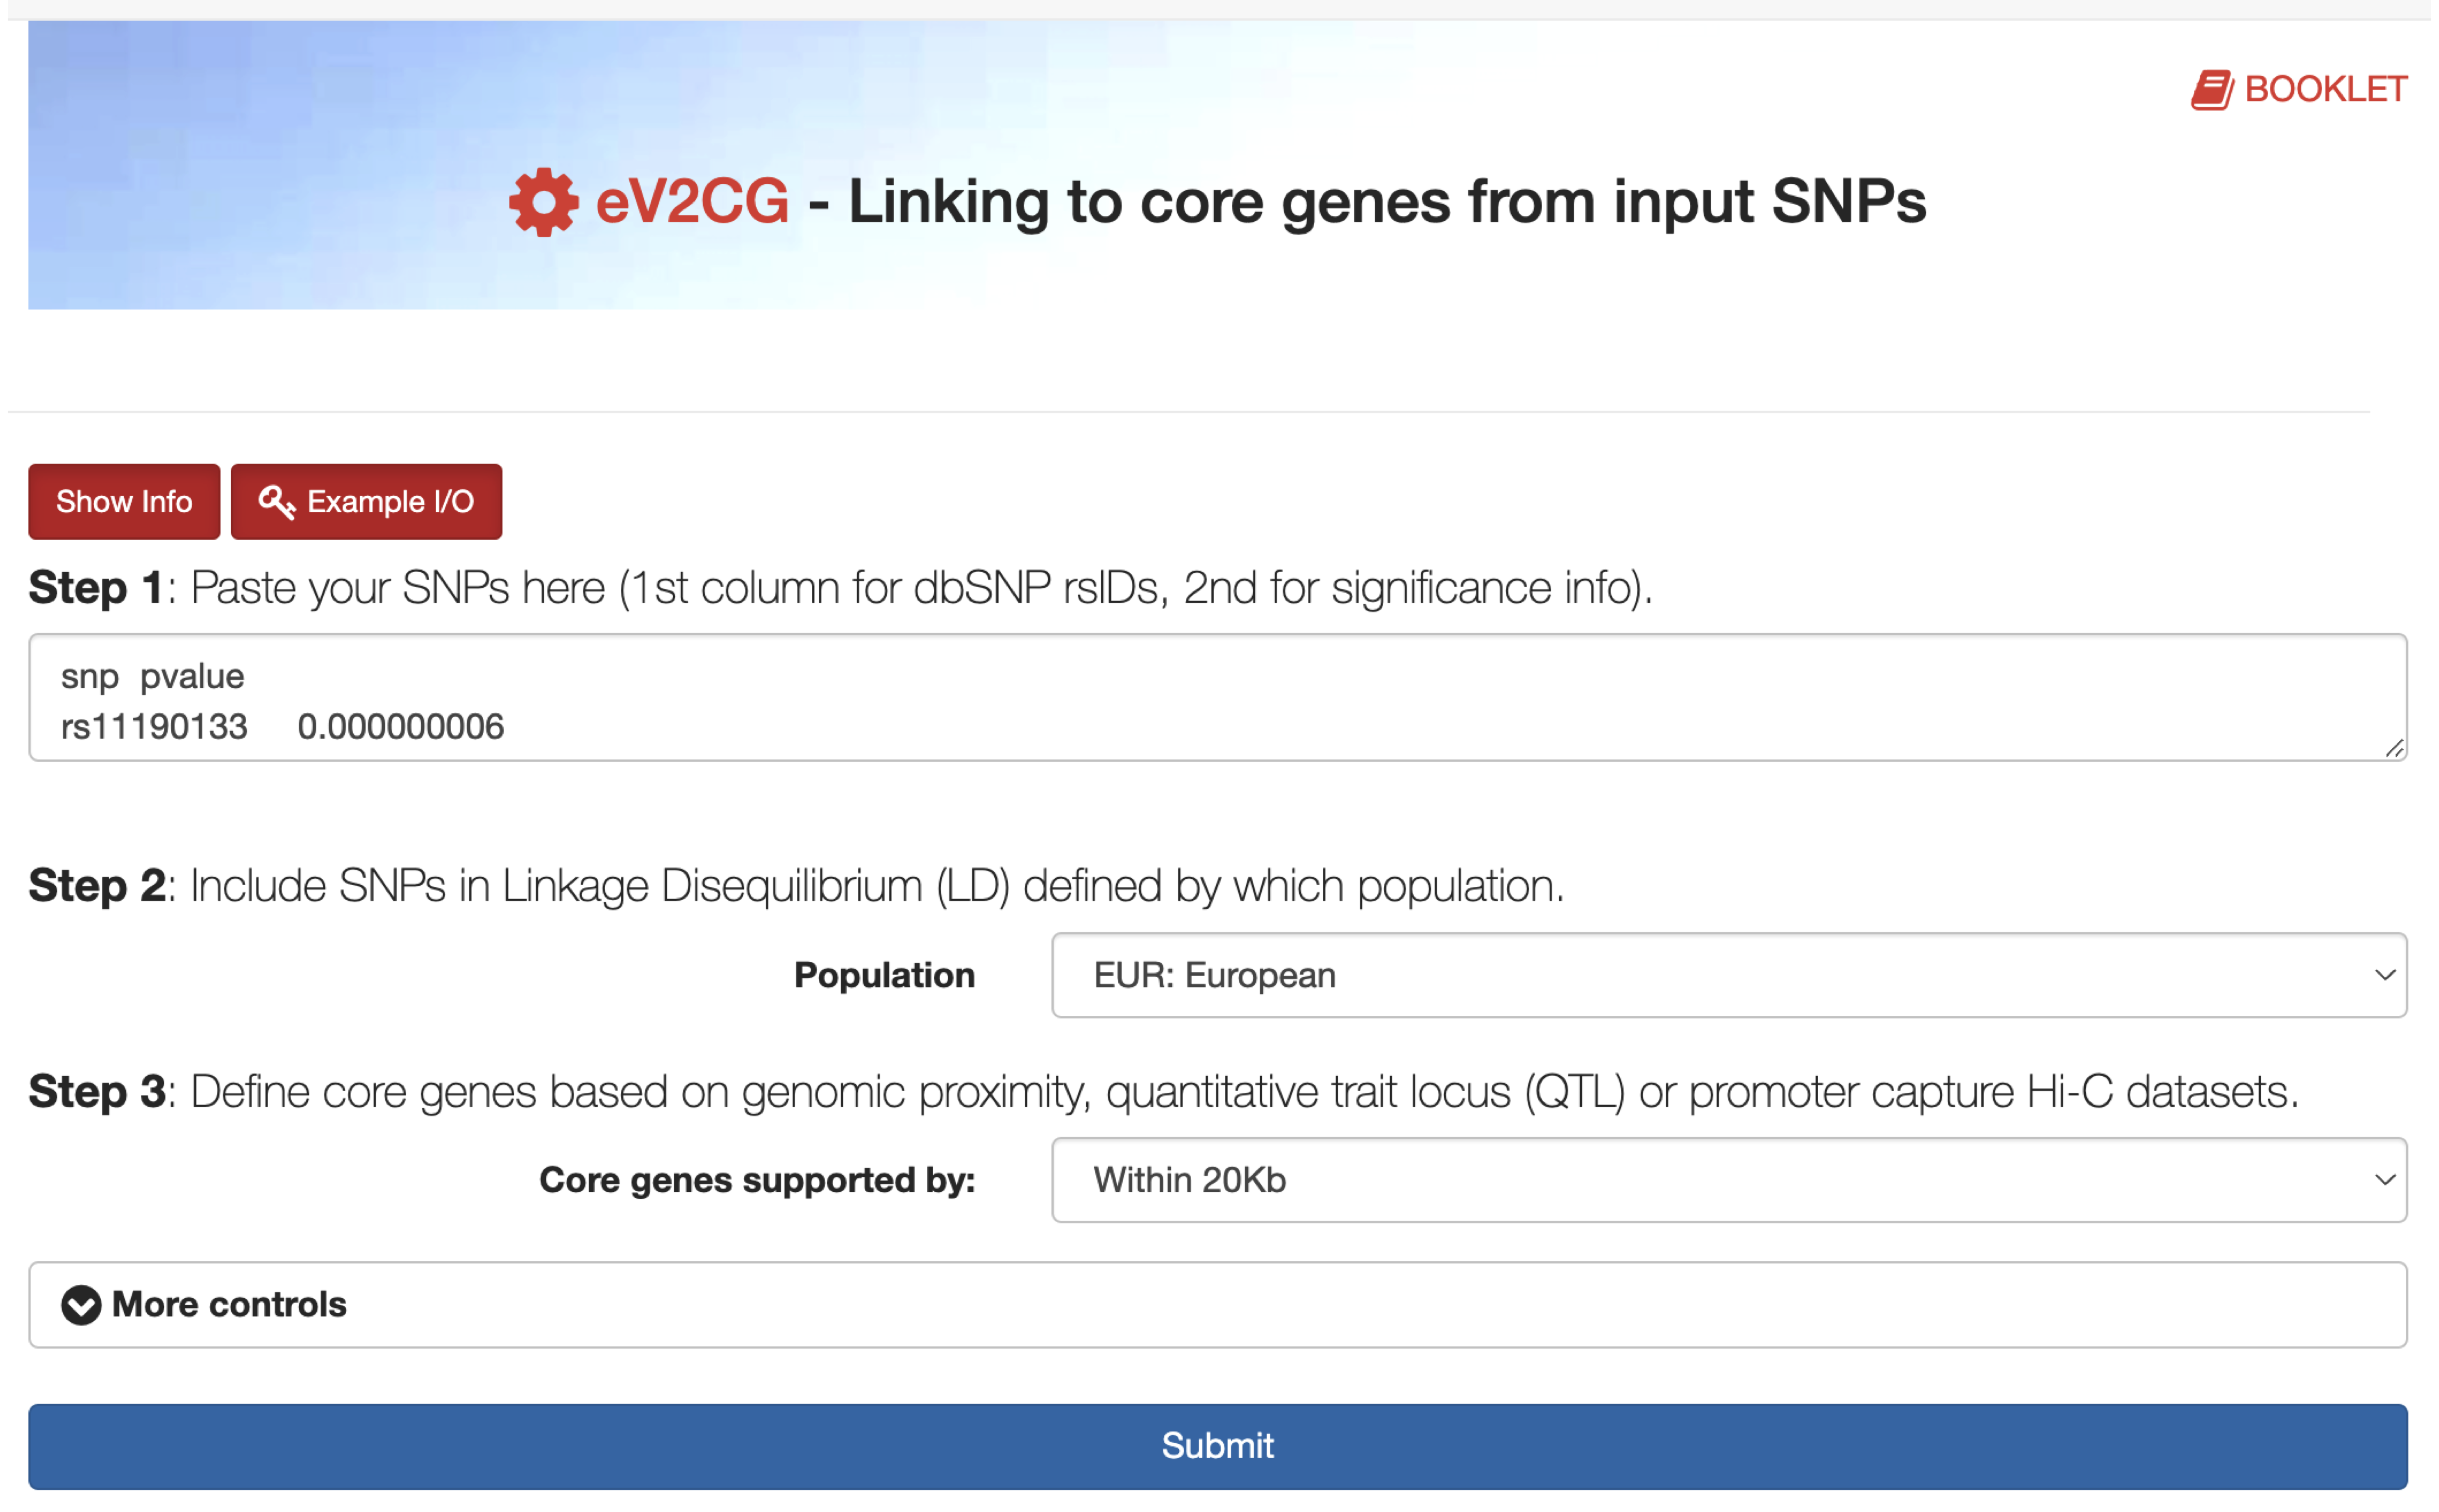
\includegraphics[width=1\linewidth]{index_files/figure-latex/eV2CG-interface-1} 

}

\caption{The interface of eV2CG, linking disease associated variants (particularly located at the non-coding genomic region) to (core) genes likely responsible for associations, based on either conformation evidence (that is, promoter-centered chromatin interactions), quantitative trait locus (QTL) mapping (that is, genetic regulation of gene expression or protein abundance), or simply genomic proximity. The Show/Hide Info toggle button contains the help information on how to use eV2CG, including input, output, mechanism, etc.}\label{fig:eV2CG-interface}
\end{figure}

\hypertarget{linking-results}{%
\section{Linking results}\label{linking-results}}

\begin{itemize}
\item
  Under the tab \texttt{Output:\ core\ genes}, \texttt{Manhattan\ plot} illustrates scored core genes that are color-coded by chromosomes. Also provided is the downloadable PDF file.
\item
  Under the tab \texttt{Output:\ core\ genes}, \texttt{An\ interactive\ table} lists core genes linked from the input SNPs, with scores quantifying the level of genes responsible for genetic associations (capped at 100). Genes are cross-referenced and linked out to GeneCards.
\end{itemize}

\begin{figure}

{\centering 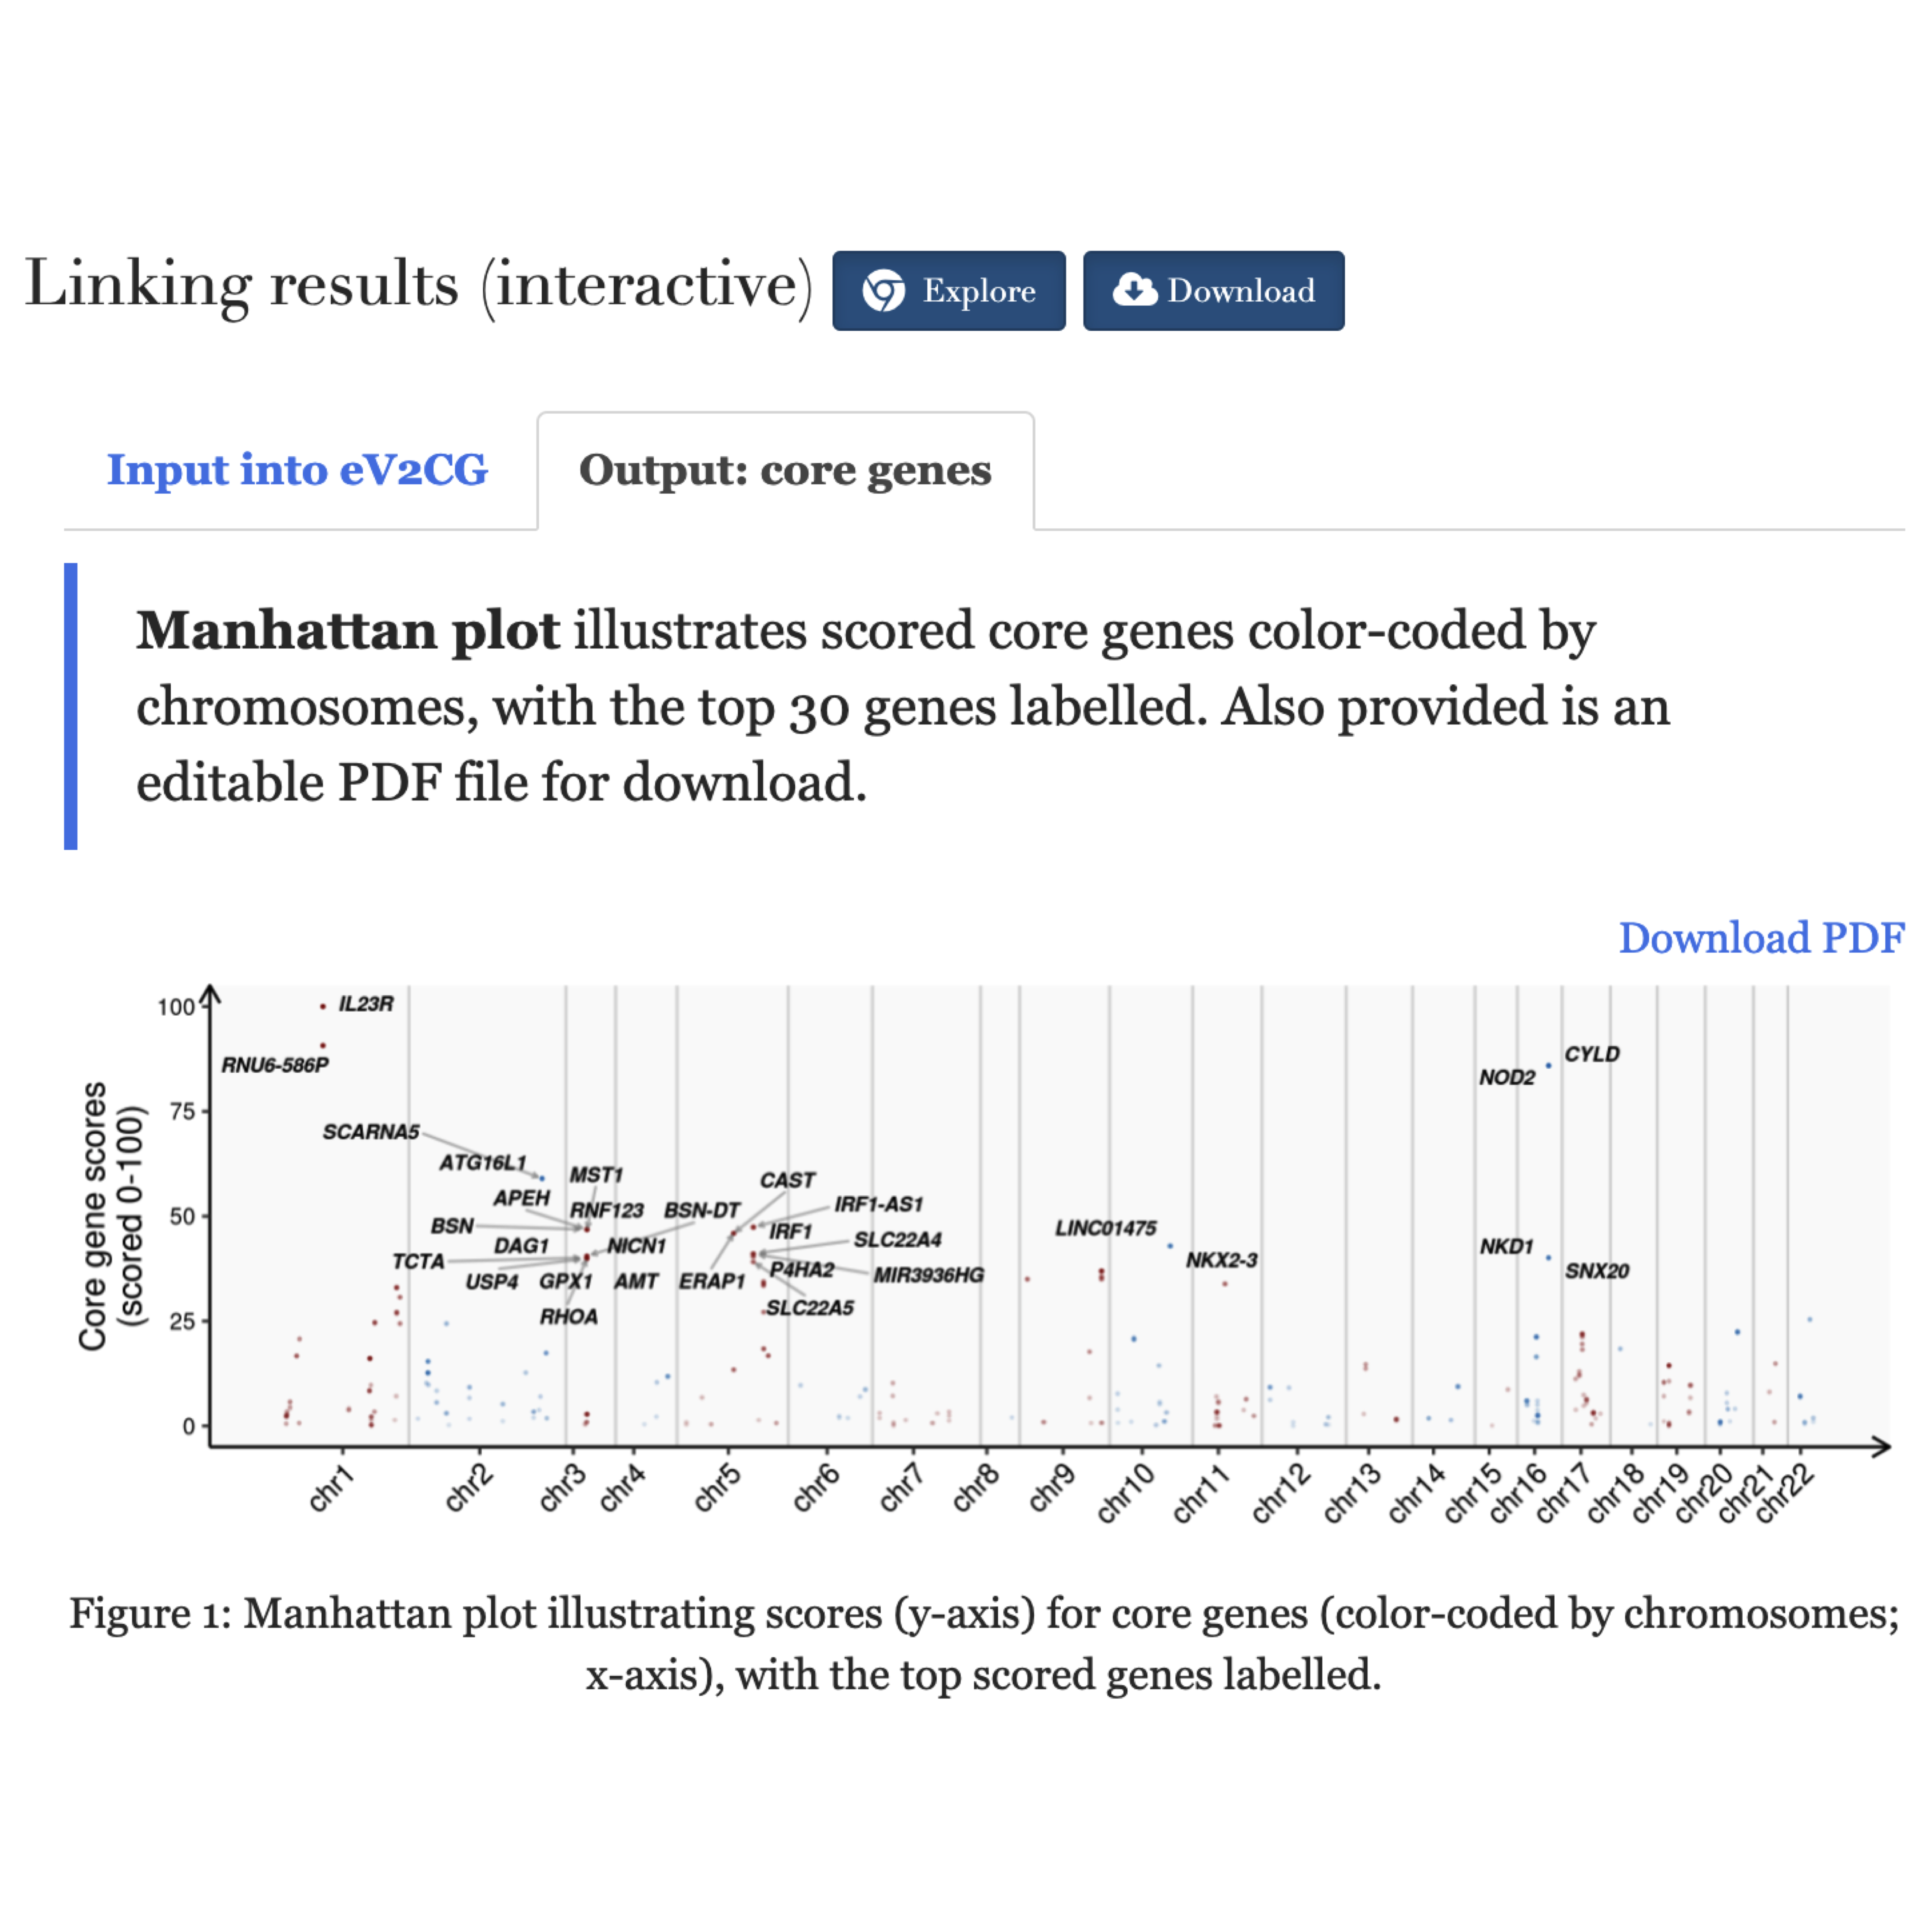
\includegraphics[width=0.7\linewidth]{index_files/figure-latex/eV2CG-results-1} 

}

\caption{Interactive results for eV2CG. The user input data are also returned for the exploration.}\label{fig:eV2CG-results}
\end{figure}

\hypertarget{ecg2pg}{%
\chapter{eCG2PG}\label{ecg2pg}}

\hypertarget{interface-1}{%
\section{Interface}\label{interface-1}}

\begin{quote}
\textbf{Input}
\end{quote}

\begin{itemize}
\tightlist
\item
  \texttt{Step\ 1}: a list of user-defined core genes (1st column for gene symbols, 2nd for weights), such as results from eV2CG above.
\end{itemize}

\begin{quote}
\textbf{Mechanism}
\end{quote}

\begin{itemize}
\item
  \texttt{Step\ 2}: networks core genes to each other and to additional (peripheral) genes based on the knowledge of protein interactions, generating a ranked list of core and peripheral genes.
\item
  \texttt{More\ controls}: fine-tunes parameters involved in steps described above.
\end{itemize}

\begin{quote}
\textbf{Output}
\end{quote}

\begin{itemize}
\tightlist
\item
  \href{http://www.genetictargets.com/app/examples/_tmp_RMD_eCG2PG.html}{Sample Output} includes an interactive table for core and peripheral genes, and a manhattan plot (illustrating scores for genes color-coded by chromosomes).
\end{itemize}

\begin{figure}

{\centering 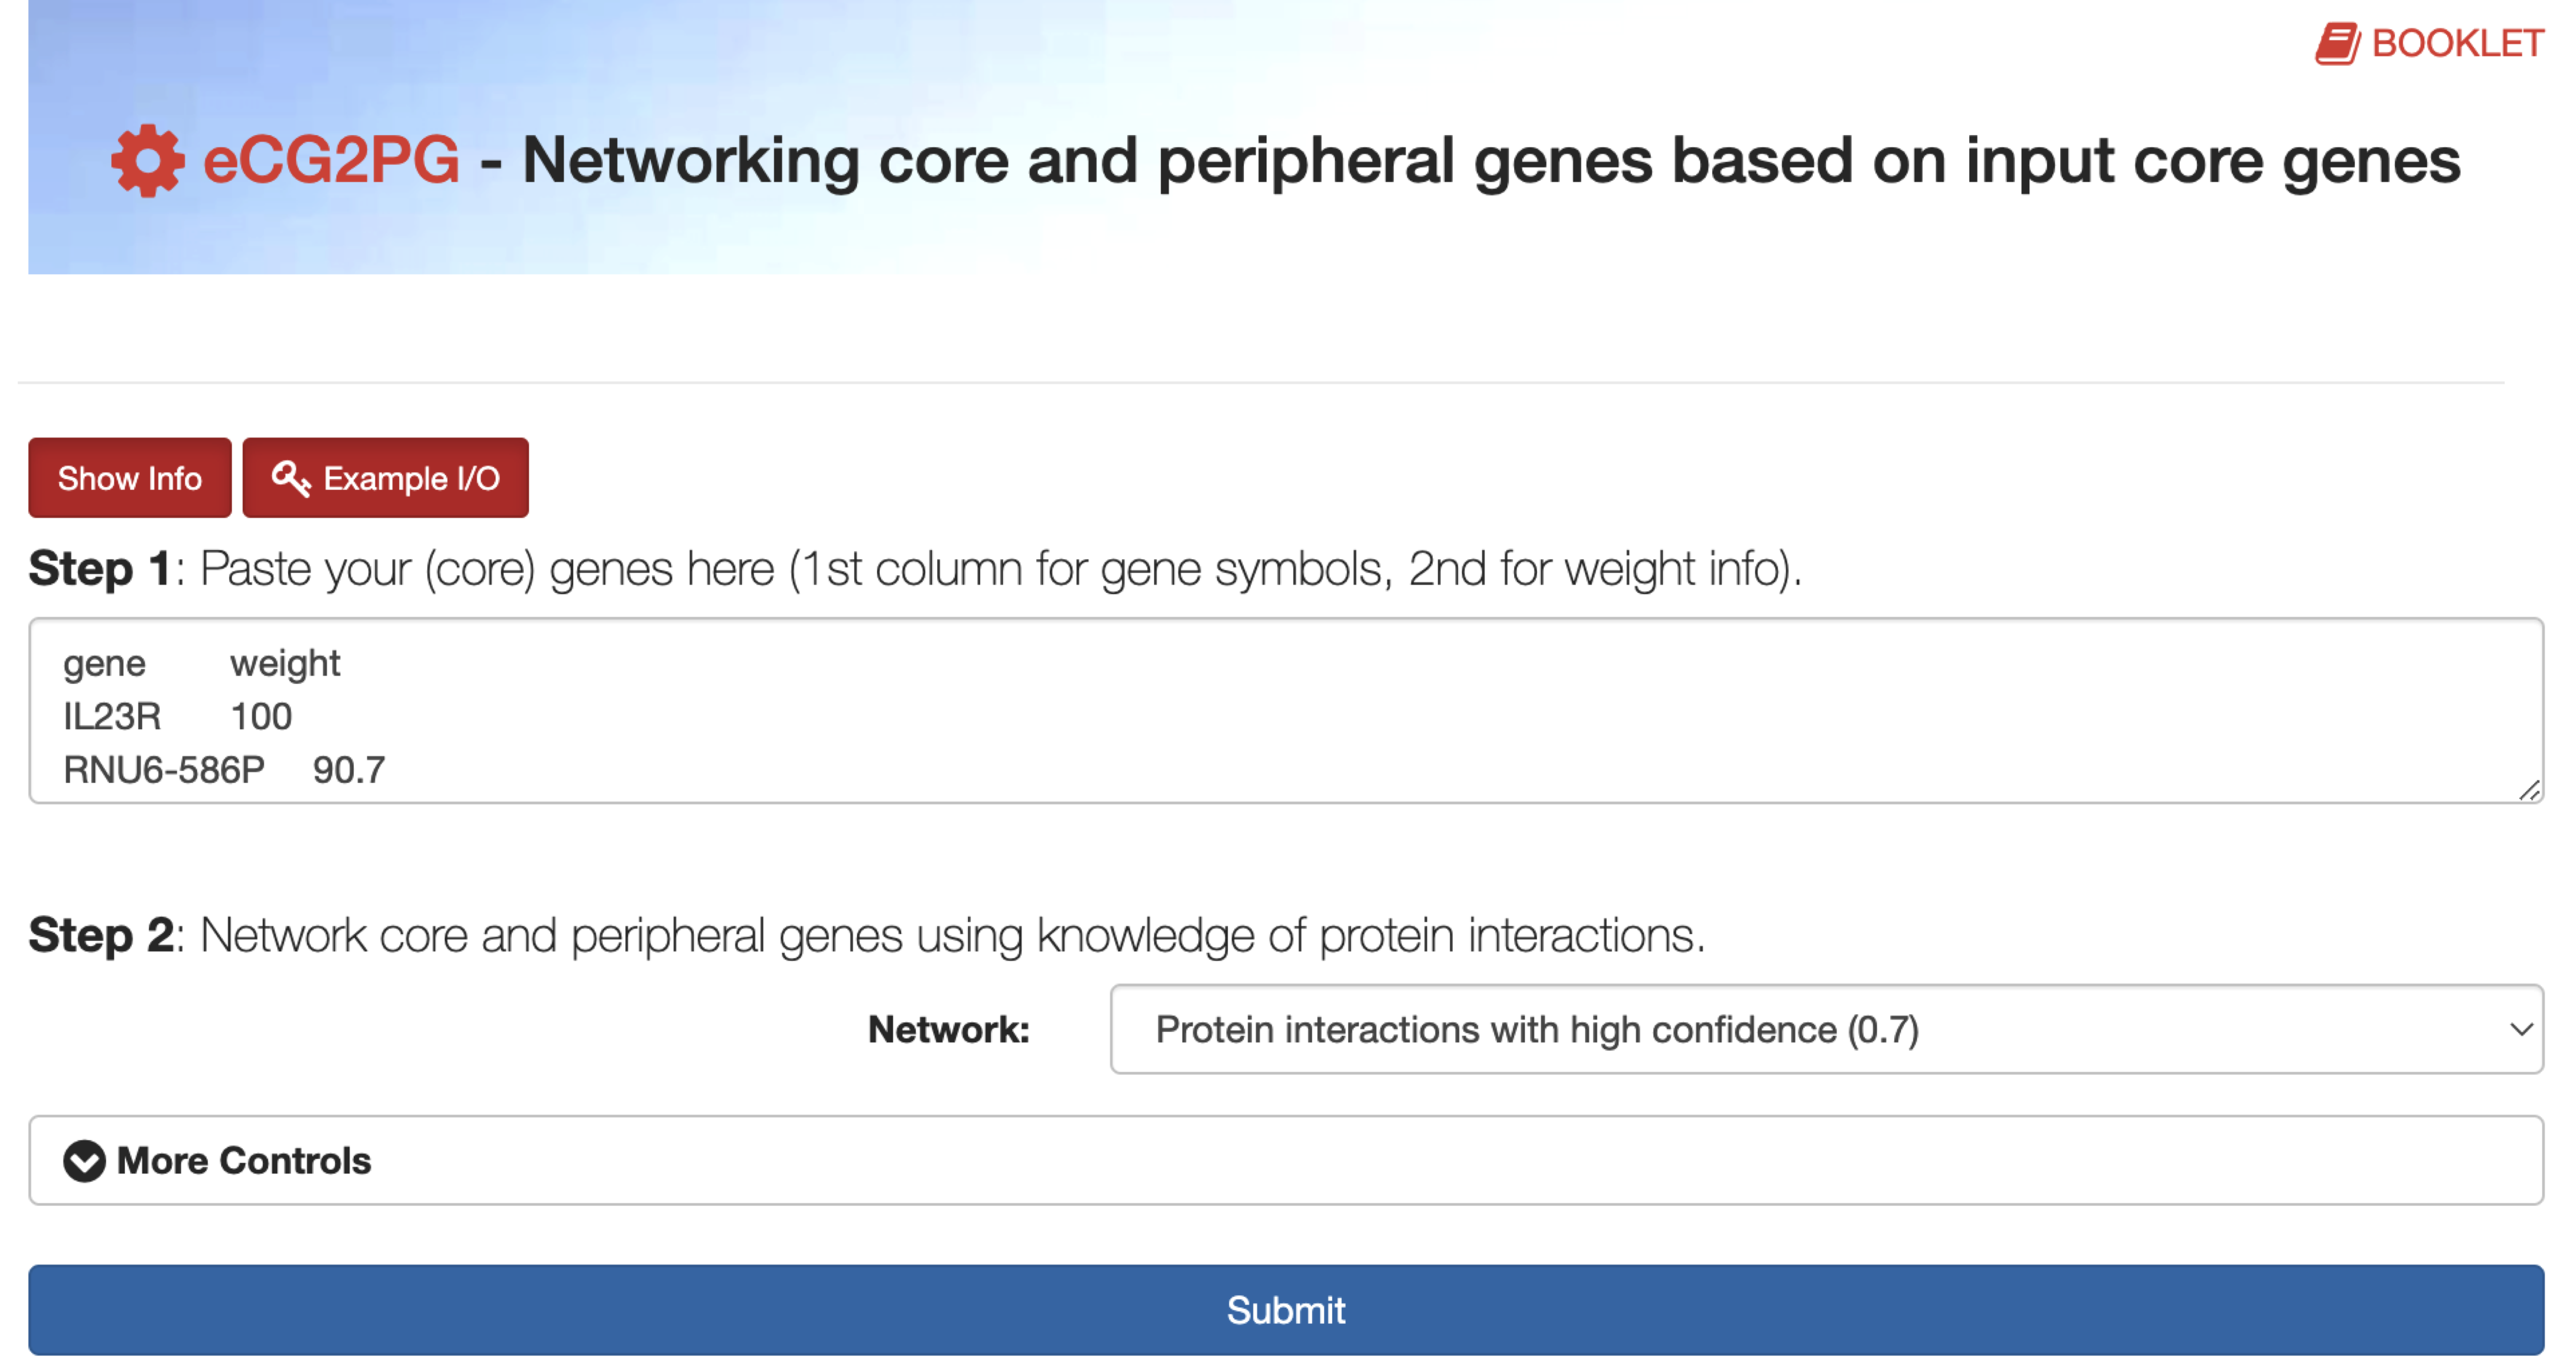
\includegraphics[width=1\linewidth]{index_files/figure-latex/eCG2PG-interface-1} 

}

\caption{The interface of eCG2PG, using the knowledge of protein interactions to ‘network’ core genes to each other and to additional (peripheral) genes as well, generating a ranked list of core and peripheral genes. The Show/Hide Info toggle button contains the help information on how to use eCG2PG, including input, output, mechanism, etc.}\label{fig:eCG2PG-interface}
\end{figure}

\hypertarget{networking-results}{%
\section{Networking results}\label{networking-results}}

\begin{itemize}
\item
  Under the tab \texttt{Output:\ core\ and\ peripheral\ genes}, \texttt{Manhattan\ plot} illustrates affinity scores for genes that are color-coded by chromosomes. Also provided is the downloadable PDF file.
\item
  Under the tab \texttt{Output:\ core\ and\ peripheral\ genes}, \texttt{An\ interactive\ table} lists core and peripheral genes, with scores quantifying the affinity to core genes (sum up to 1). Genes are cross-referenced and linked out to GeneCards.
\end{itemize}

\begin{figure}

{\centering 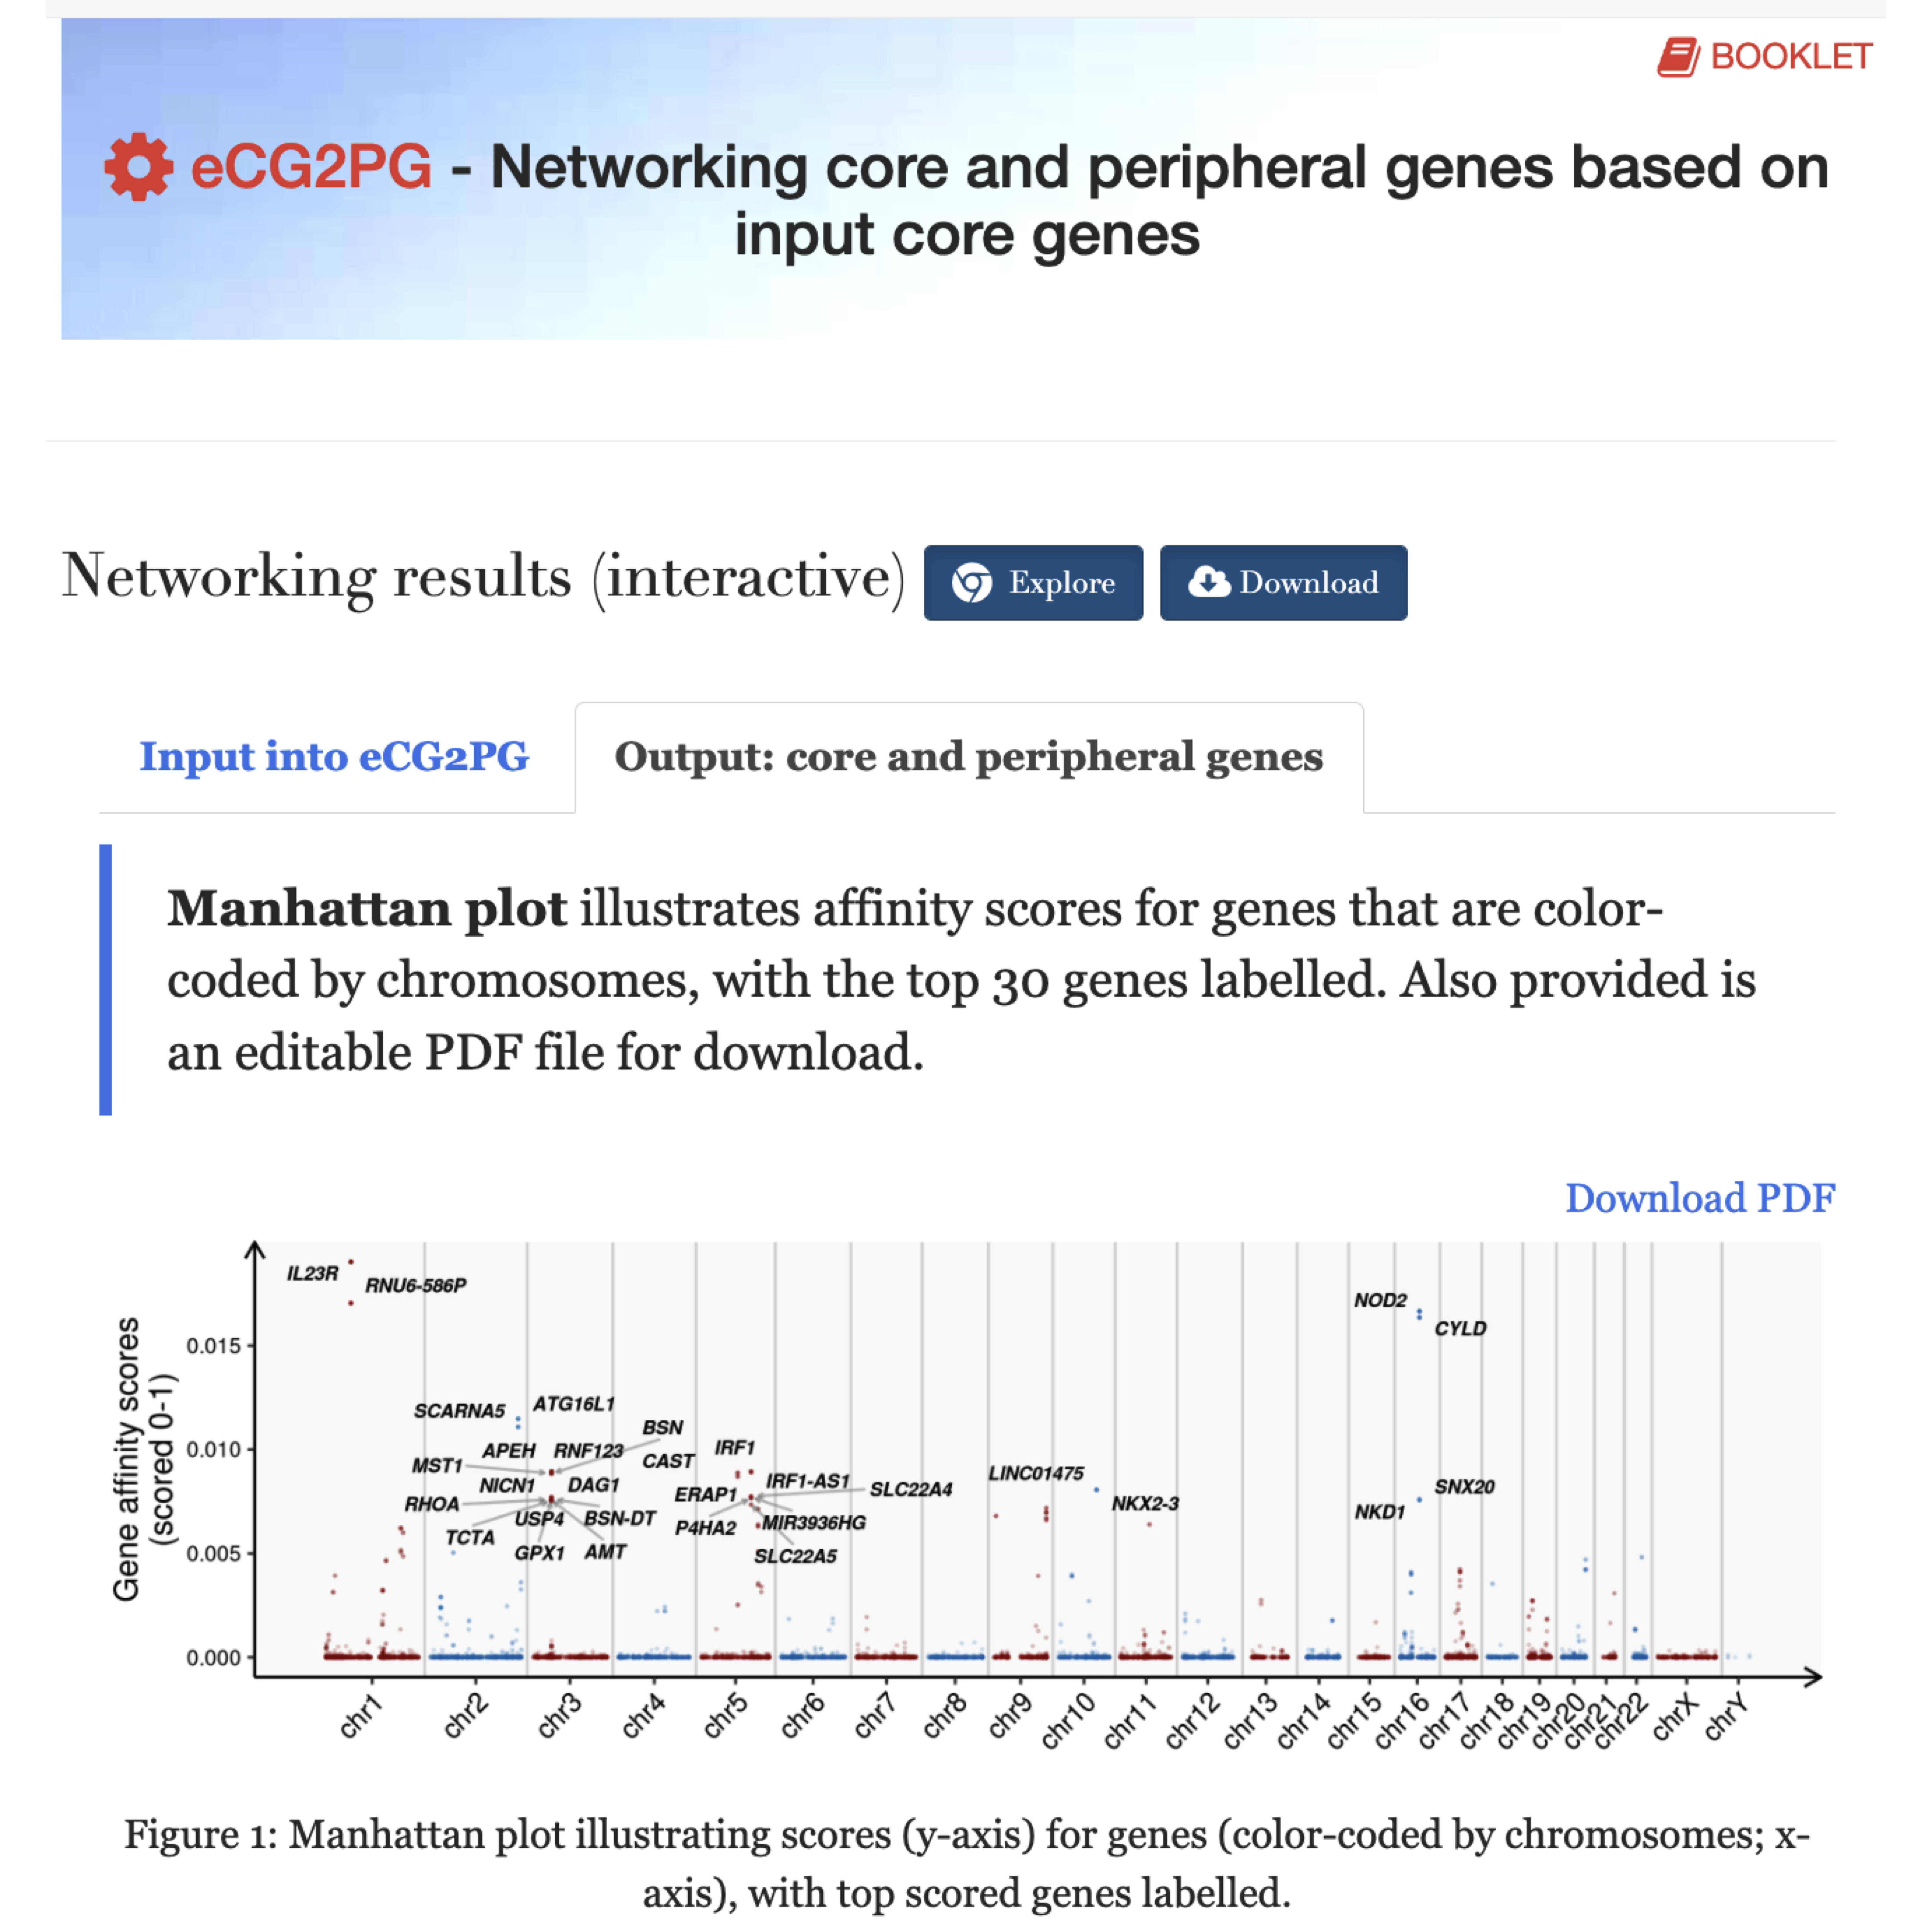
\includegraphics[width=0.7\linewidth]{index_files/figure-latex/eCG2PG-results-1} 

}

\caption{Interactive results for eCG2PG. The user input data are also returned for the exploration.}\label{fig:eCG2PG-results}
\end{figure}

\hypertarget{ecrosstalk}{%
\chapter{eCrosstalk}\label{ecrosstalk}}

\hypertarget{interface-2}{%
\section{Interface}\label{interface-2}}

\begin{quote}
\textbf{Input}
\end{quote}

\begin{itemize}
\tightlist
\item
  \texttt{Step\ 1}: a ranked list of genes (1st column for gene symbols, 2nd for scores), such as results from eCG2PG above.
\end{itemize}

\begin{quote}
\textbf{Mechanism}
\end{quote}

\begin{itemize}
\tightlist
\item
  \texttt{Step\ 2}: identifies the subnetwork of highly ranked genes that mediate pathway crosstalk.
\end{itemize}

\begin{quote}
\textbf{Output}
\end{quote}

\begin{itemize}
\tightlist
\item
  \href{http://www.genetictargets.com/app/examples/_tmp_RMD_eCrosstalk.html}{Sample Output} includes an interactive table for pathway crosstalk genes, and a network visualisation (illustrating the crosstalk between pathways).
\end{itemize}

\begin{figure}

{\centering 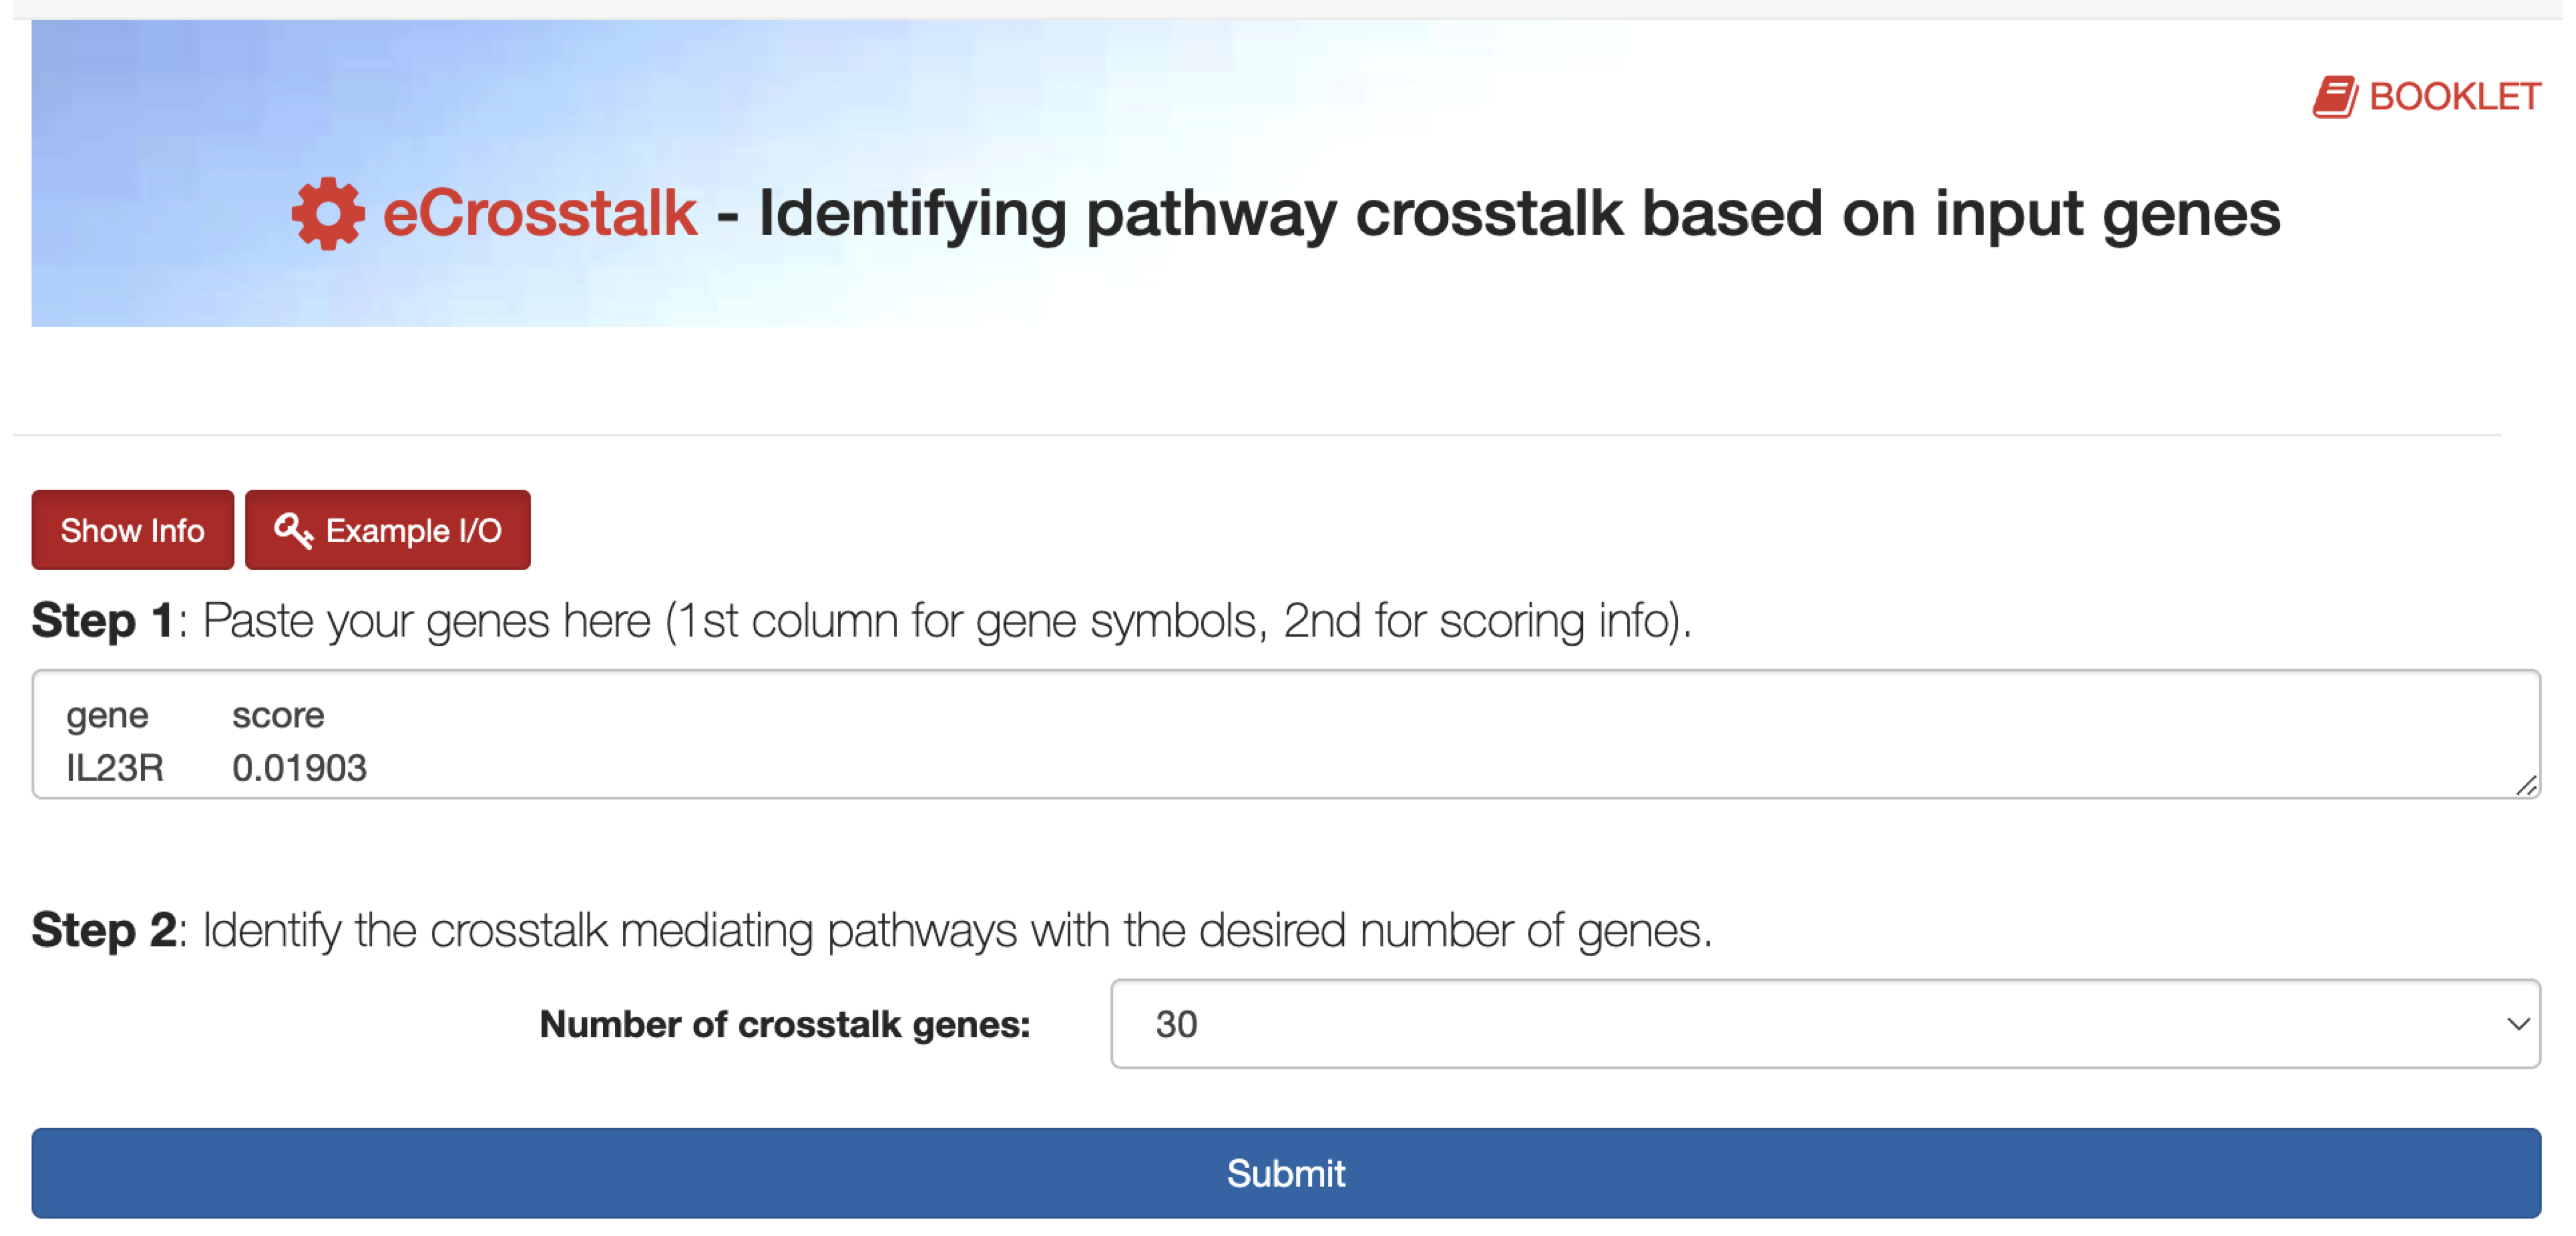
\includegraphics[width=1\linewidth]{index_files/figure-latex/eCrosstalk-interface-1} 

}

\caption{The interface of eCrosstalk, exploiting the information of well-curated pathway-derived interactions to identify the subnetwork of highly ranked genes that mediate pathway crosstalk. The Show/Hide Info toggle button introducing how to use eCrosstalk, including input, output, mechanism, etc.}\label{fig:eCrosstalk-interface}
\end{figure}

\hypertarget{crosstalk-results}{%
\section{Crosstalk results}\label{crosstalk-results}}

\begin{itemize}
\item
  Under the tab \texttt{Output:\ pathway\ crosstalk}, \texttt{A\ network\ visualisation} illustrates crosstalk genes color-coded by input scores. Also provided is the downloadable PDF file.
\item
  Under the tab \texttt{Output:\ pathway\ crosstalk}, \texttt{An\ interactive\ table}: lists crosstalk genes together with input scores. Genes are cross-referenced and linked out to GeneCards.
\end{itemize}

\begin{figure}

{\centering 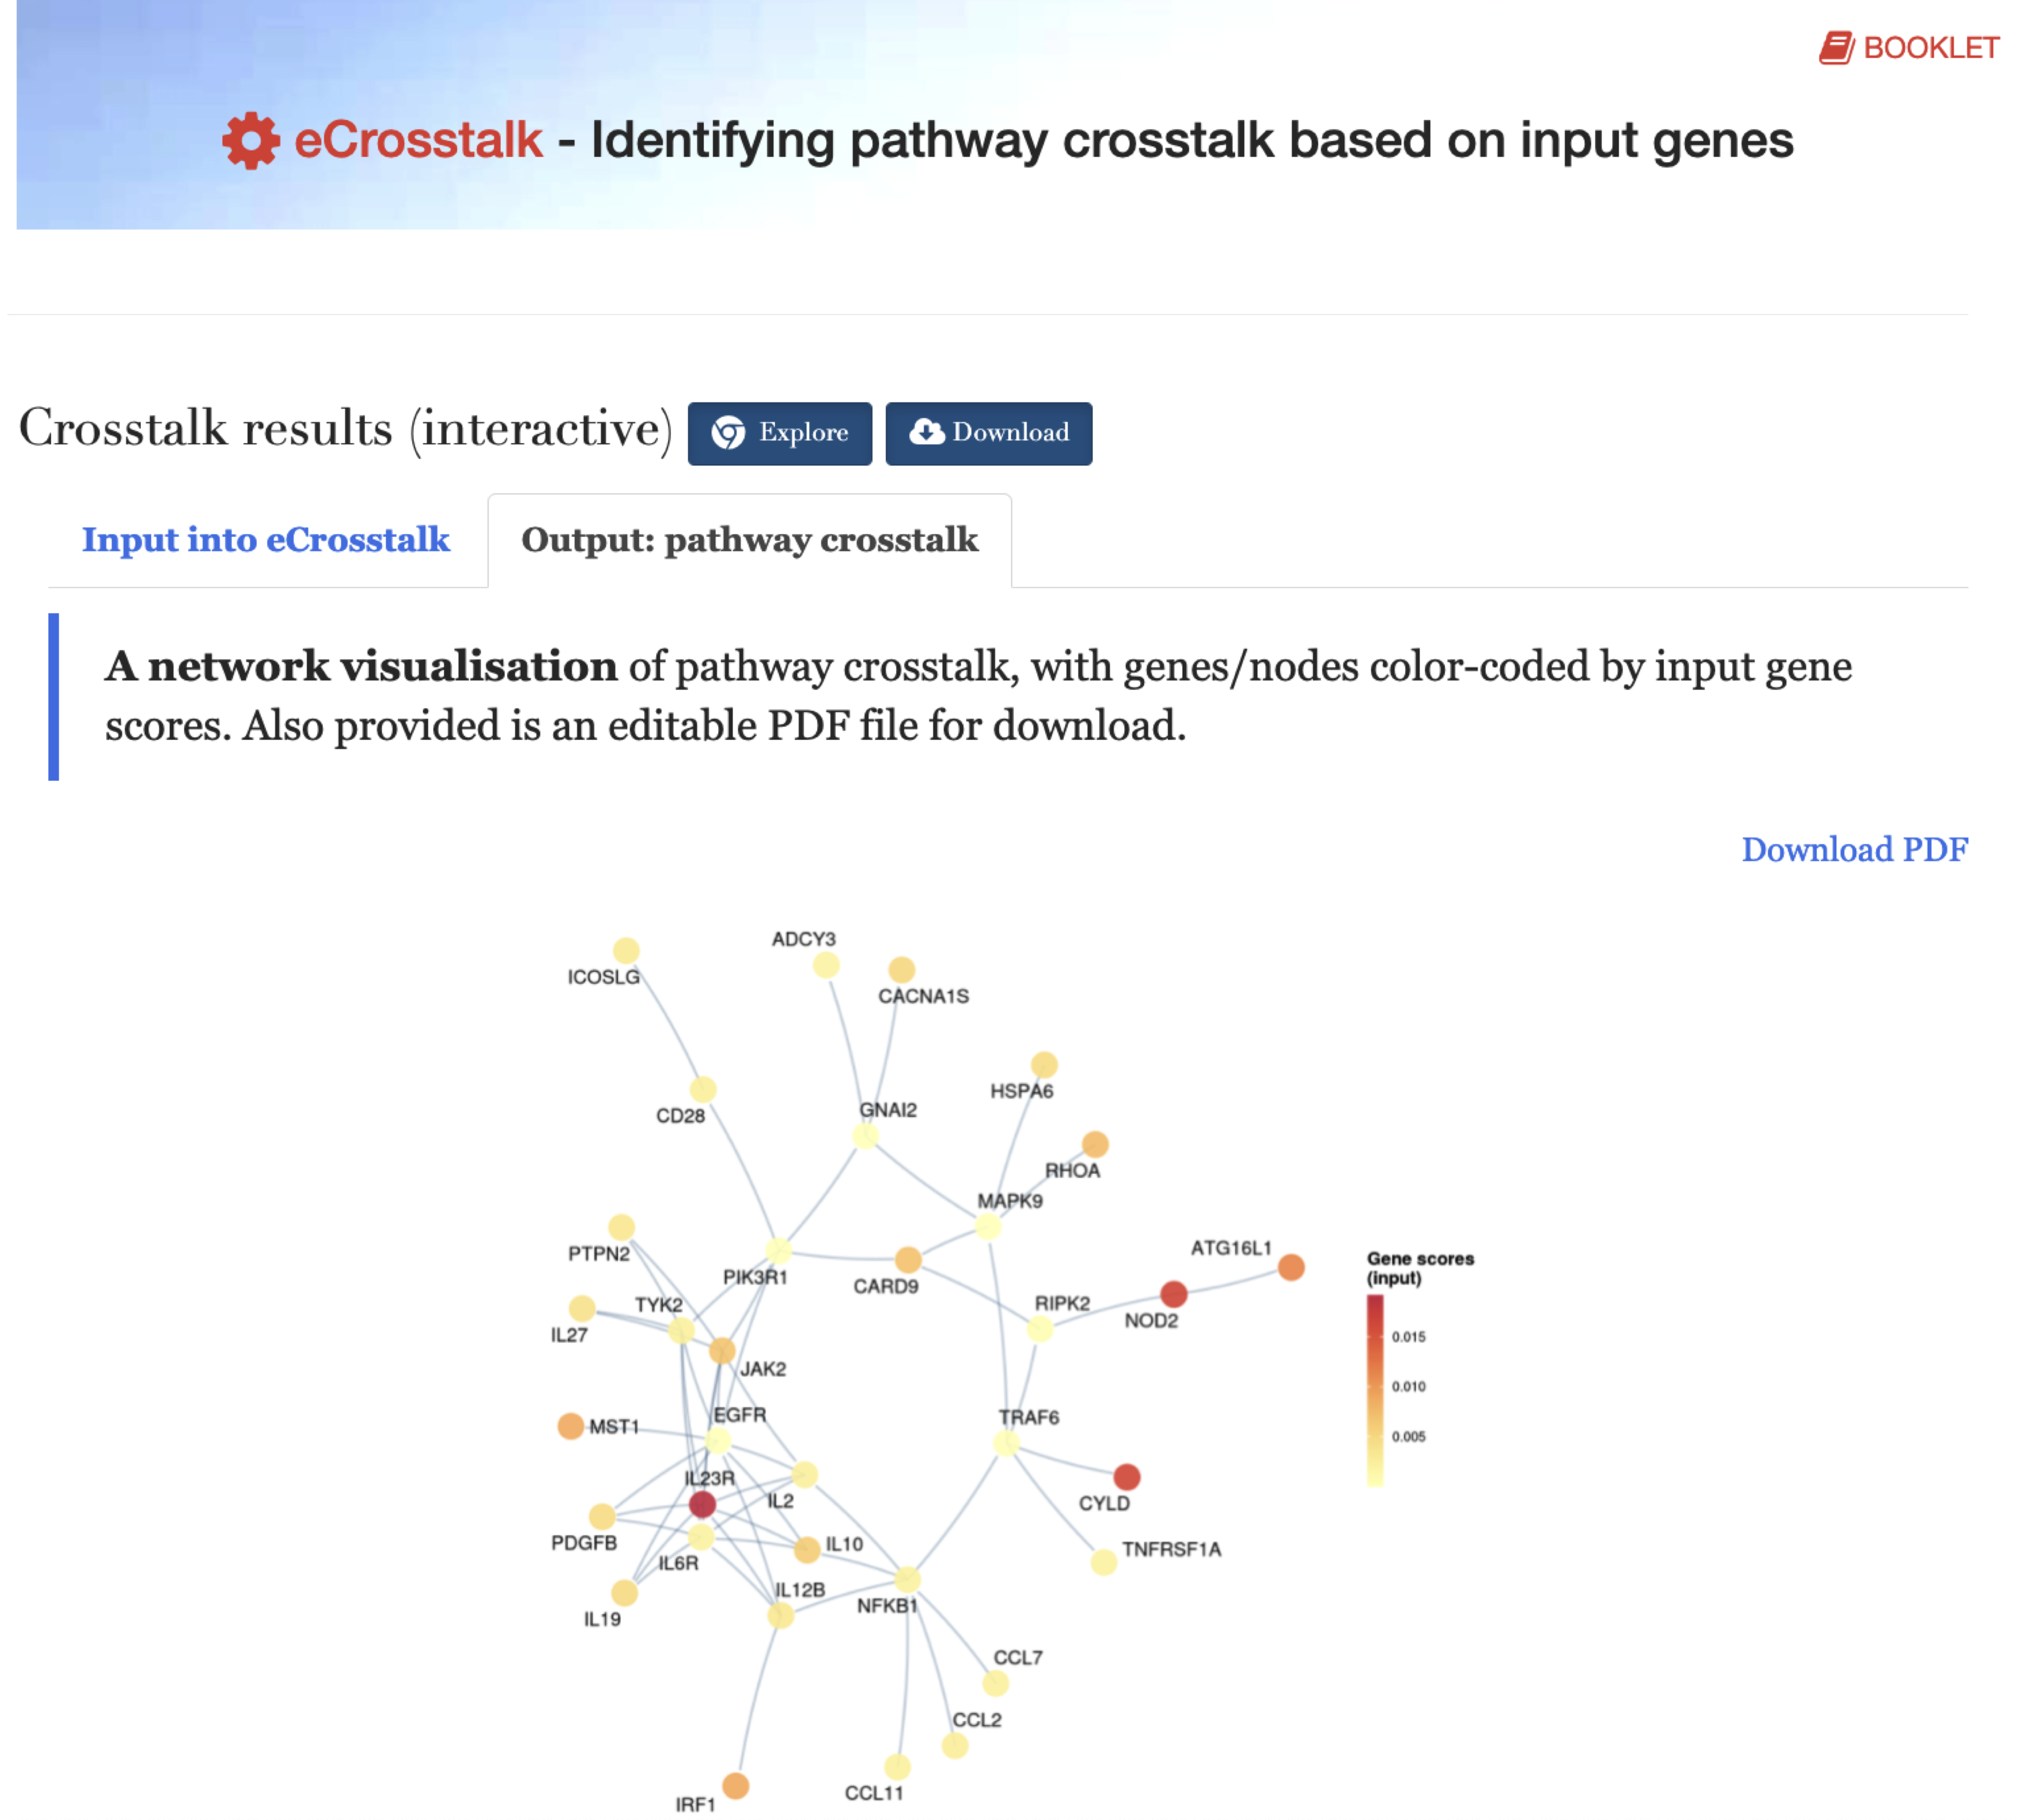
\includegraphics[width=1\linewidth]{index_files/figure-latex/eCrosstalk-results-1} 

}

\caption{Interactive results for eCrosstalk. The user input data are also returned for the exploration.}\label{fig:eCrosstalk-results}
\end{figure}

\hypertarget{ctgene}{%
\chapter{cTGene}\label{ctgene}}

\hypertarget{interface-3}{%
\section{Interface}\label{interface-3}}

\begin{quote}
\textbf{Input}
\end{quote}

\begin{itemize}
\tightlist
\item
  \texttt{Step\ 1}: a list of user-defined SNPs (1st column for dbSNP rsIDs, 2nd for significance info). By default, sample data are shared genetic variants identified from cross-disease genome-wide association studies in inflammatory disorders; see \href{https://www.ncbi.nlm.nih.gov/pubmed/26974007}{Nature Genetics 2016}.
\end{itemize}

\begin{quote}
\textbf{Mechanism}
\end{quote}

\begin{itemize}
\item
  \texttt{Step\ 2}: includes SNPs in Linkage Disequilibrium (LD).
\item
  \texttt{Step\ 3}: uses genomic proximity, quantitative trait locus (QTL), or promoter capture Hi-C data to identify core genes.
\item
  \texttt{Step\ 4}: networks core genes to each other and to additional (peripheral) genes based on the knowledge of protein interactions, generating a ranked list of core and peripheral genes.
\item
  \texttt{More\ controls}: fine-tunes parameters involved in steps described above.
\end{itemize}

\begin{quote}
\textbf{Output}
\end{quote}

\begin{itemize}
\tightlist
\item
  \href{http://www.genetictargets.com/app/examples/_tmp_RMD_cTGene.html}{Sample Output} includes an interactive table for targets at the gene level, and a manhattan plot (illustrating priority rating for target genes color-coded by chromosomes).
\end{itemize}

\begin{figure}

{\centering 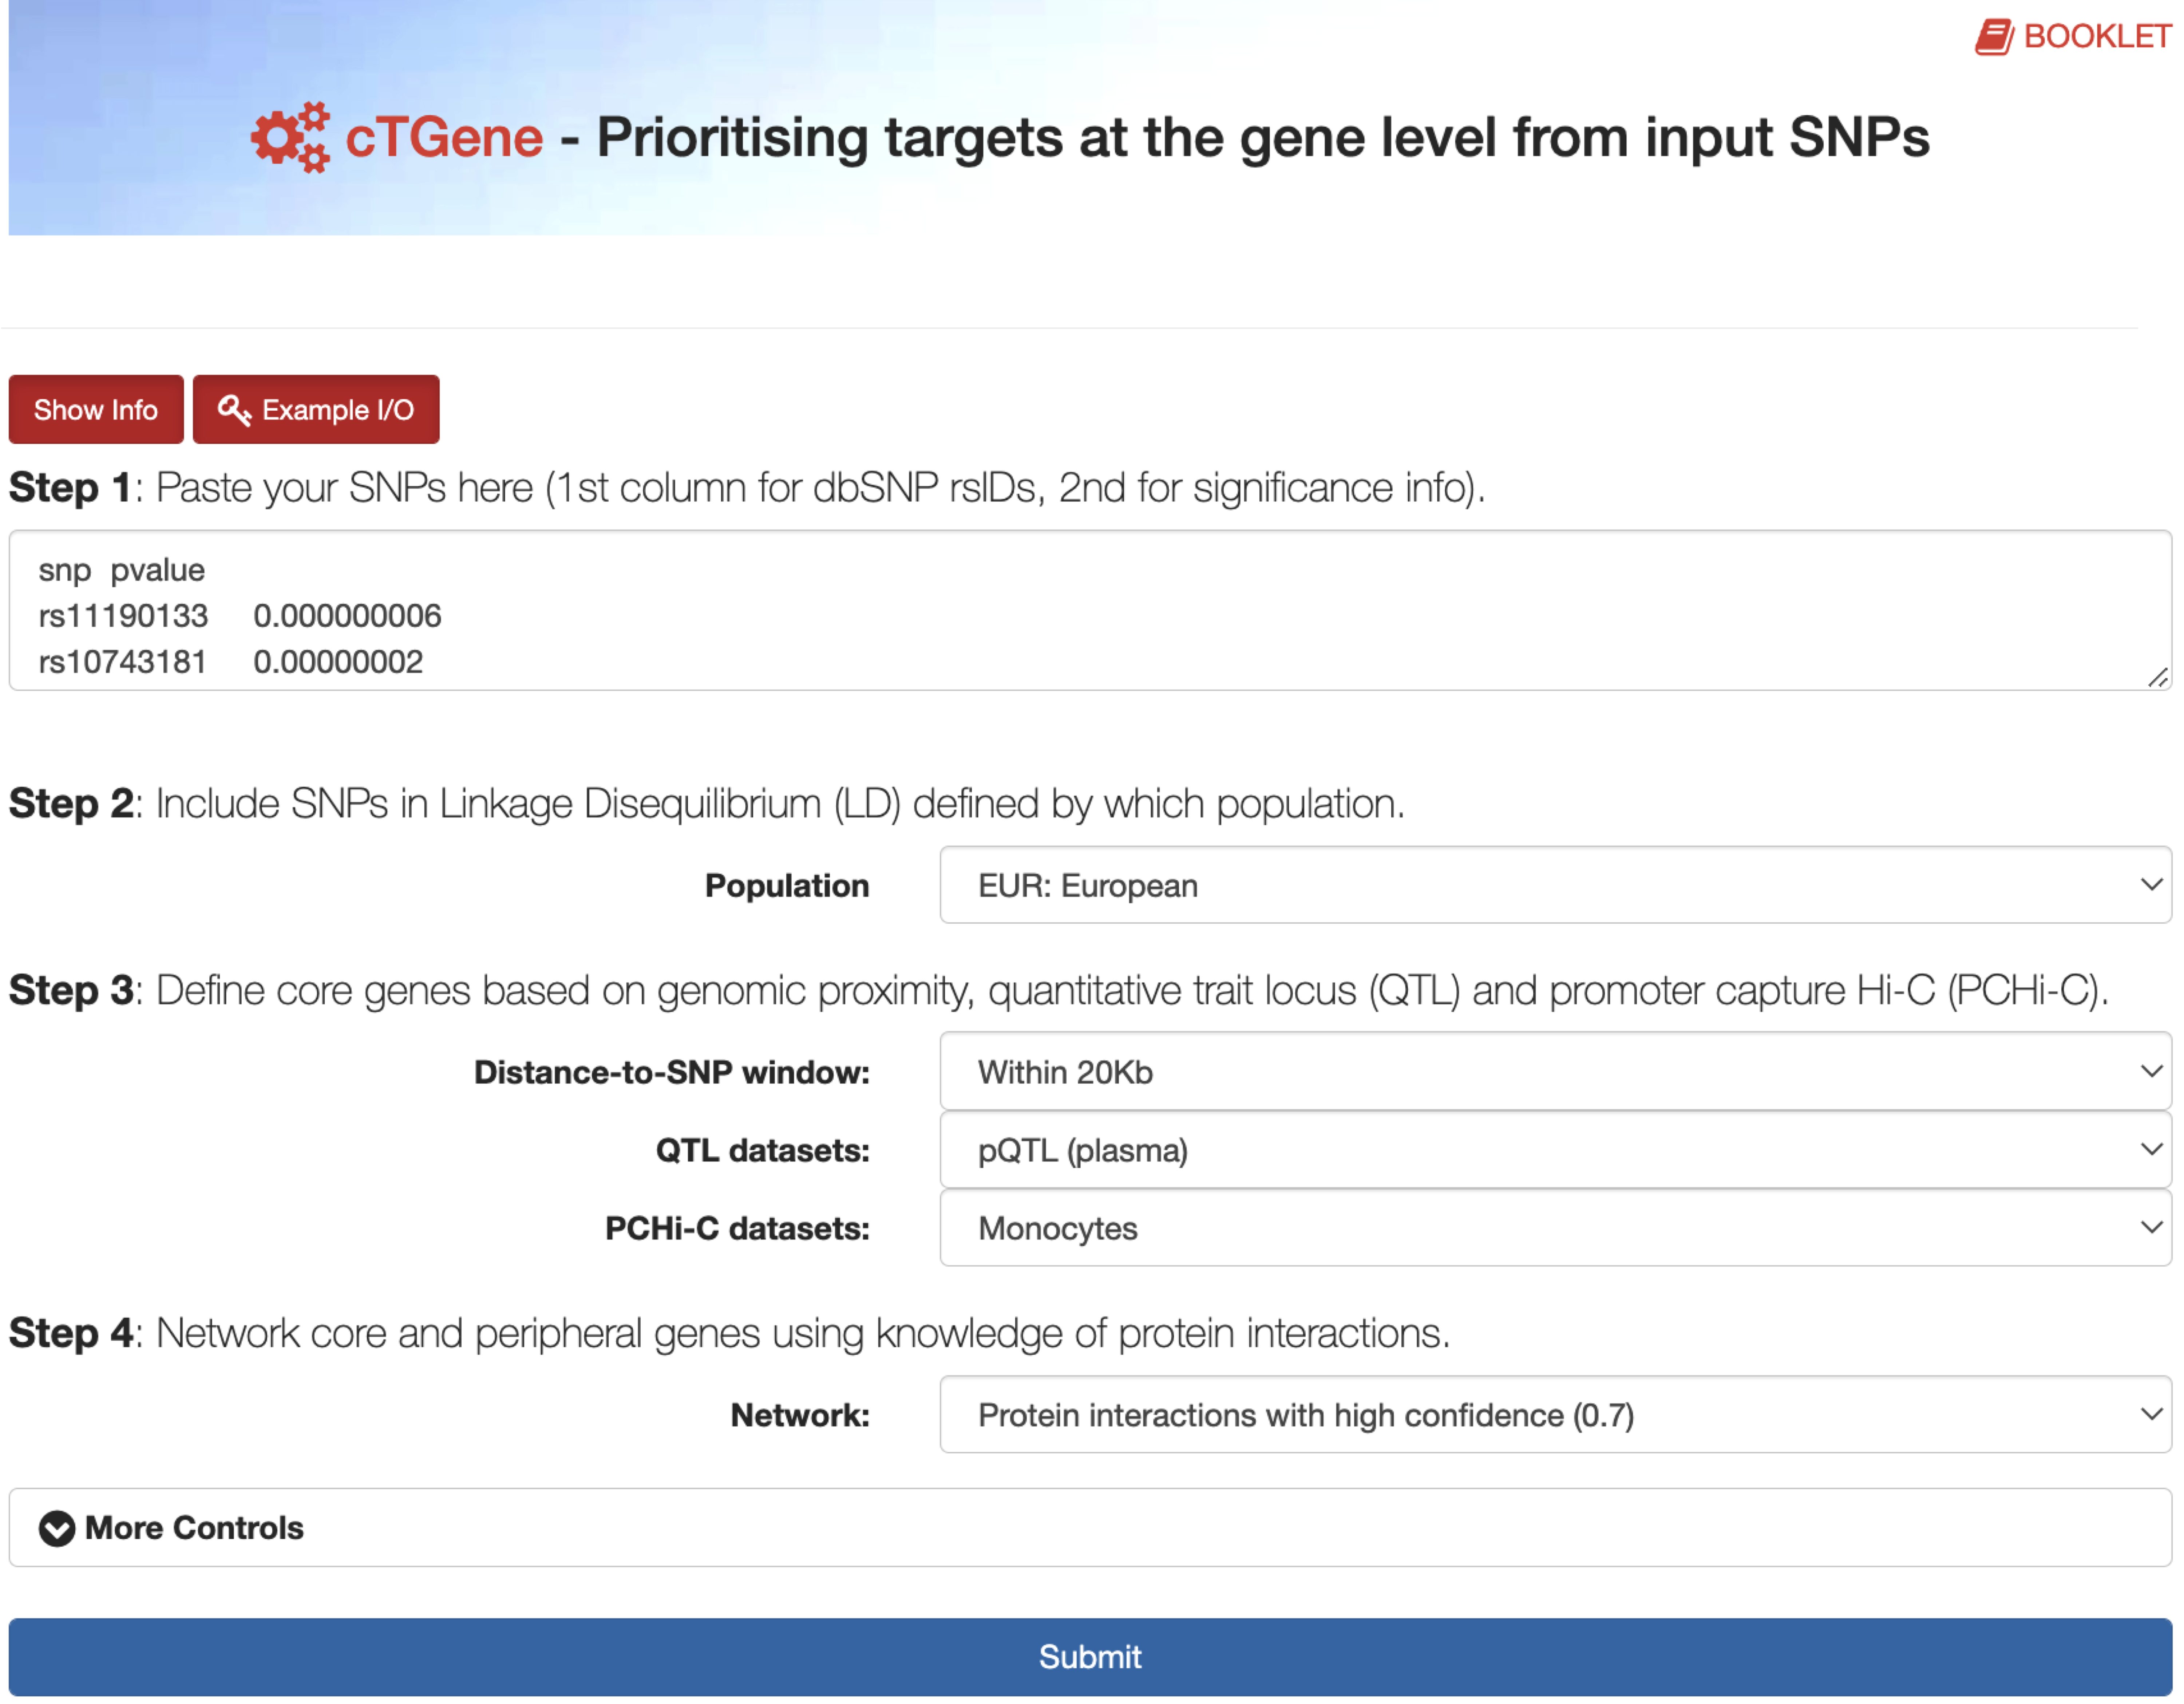
\includegraphics[width=1\linewidth]{index_files/figure-latex/cTGene-interface-1} 

}

\caption{The interface of cTGene, enabling/automating genetics-led and network-based identification and prioritisation of drug targets at the gene level. The Show/Hide Info toggle button contains the help information on how to use cTGene, including input, output, mechanism, etc.}\label{fig:cTGene-interface}
\end{figure}

\hypertarget{prioritisation-results}{%
\section{Prioritisation results}\label{prioritisation-results}}

\begin{itemize}
\item
  Under the tab \texttt{Output:\ target\ genes}, \texttt{Manhattan\ plot} illustrates priority rating for target genes that are color-coded by chromosomes. Also provided is the downloadable PDF file.
\item
  Under the tab \texttt{Output:\ target\ genes}, \texttt{An\ interactive\ table} lists all prioritised genes, each receiving 5-star priority rating (scored 0-5). Genes are cross-referenced and linked out to GeneCards.
\end{itemize}

\begin{figure}

{\centering \includegraphics[width=1\linewidth]{index_files/figure-latex/cTGene-results-1} 

}

\caption{Interactive results for cTGene. The user input data are also returned for the exploration.}\label{fig:cTGene-results}
\end{figure}

\hypertarget{ctcrosstalk}{%
\chapter{cTCrosstalk}\label{ctcrosstalk}}

\hypertarget{interface-4}{%
\section{Interface}\label{interface-4}}

\begin{quote}
\textbf{Input}
\end{quote}

\begin{itemize}
\tightlist
\item
  \texttt{Step\ 1}: a list of user-defined SNPs (1st column for dbSNP rsIDs, 2nd for significance info). By default, sample data are shared genetic variants identified from cross-disease genome-wide association studies in inflammatory disorders; see \href{https://www.ncbi.nlm.nih.gov/pubmed/26974007}{Nature Genetics 2016}.
\end{itemize}

\begin{quote}
\textbf{Mechanism}
\end{quote}

\begin{itemize}
\item
  \texttt{Step\ 2}: includes SNPs in Linkage Disequilibrium (LD).
\item
  \texttt{Step\ 3}: uses genomic proximity, quantitative trait locus (QTL), or promoter capture Hi-C data to identify core genes.
\item
  \texttt{Step\ 4}: networks core genes to each other and to additional (peripheral) genes based on the knowledge of protein interactions, generating a ranked list of core and peripheral genes.
\item
  \texttt{Step\ 5}: identifies the subnetwork of highly ranked genes that mediate pathway crosstalk.
\item
  \texttt{More\ controls}: fine-tunes parameters involved in steps described above.
\end{itemize}

\begin{quote}
\textbf{Output}
\end{quote}

\begin{itemize}
\tightlist
\item
  \href{http://www.genetictargets.com/app/examples/_tmp_RMD_cTCrosstalk.html}{Sample Output} includes an interactive table for targets at the gene level, a manhattan plot illustrating priority rating for target genes color-coded by chromosomes, a dot plot and an interactive table for target pathways, an interactive table for pathway crosstalk genes, and a network visualisation illustrating the crosstalk between pathways.
\end{itemize}

\begin{figure}

{\centering 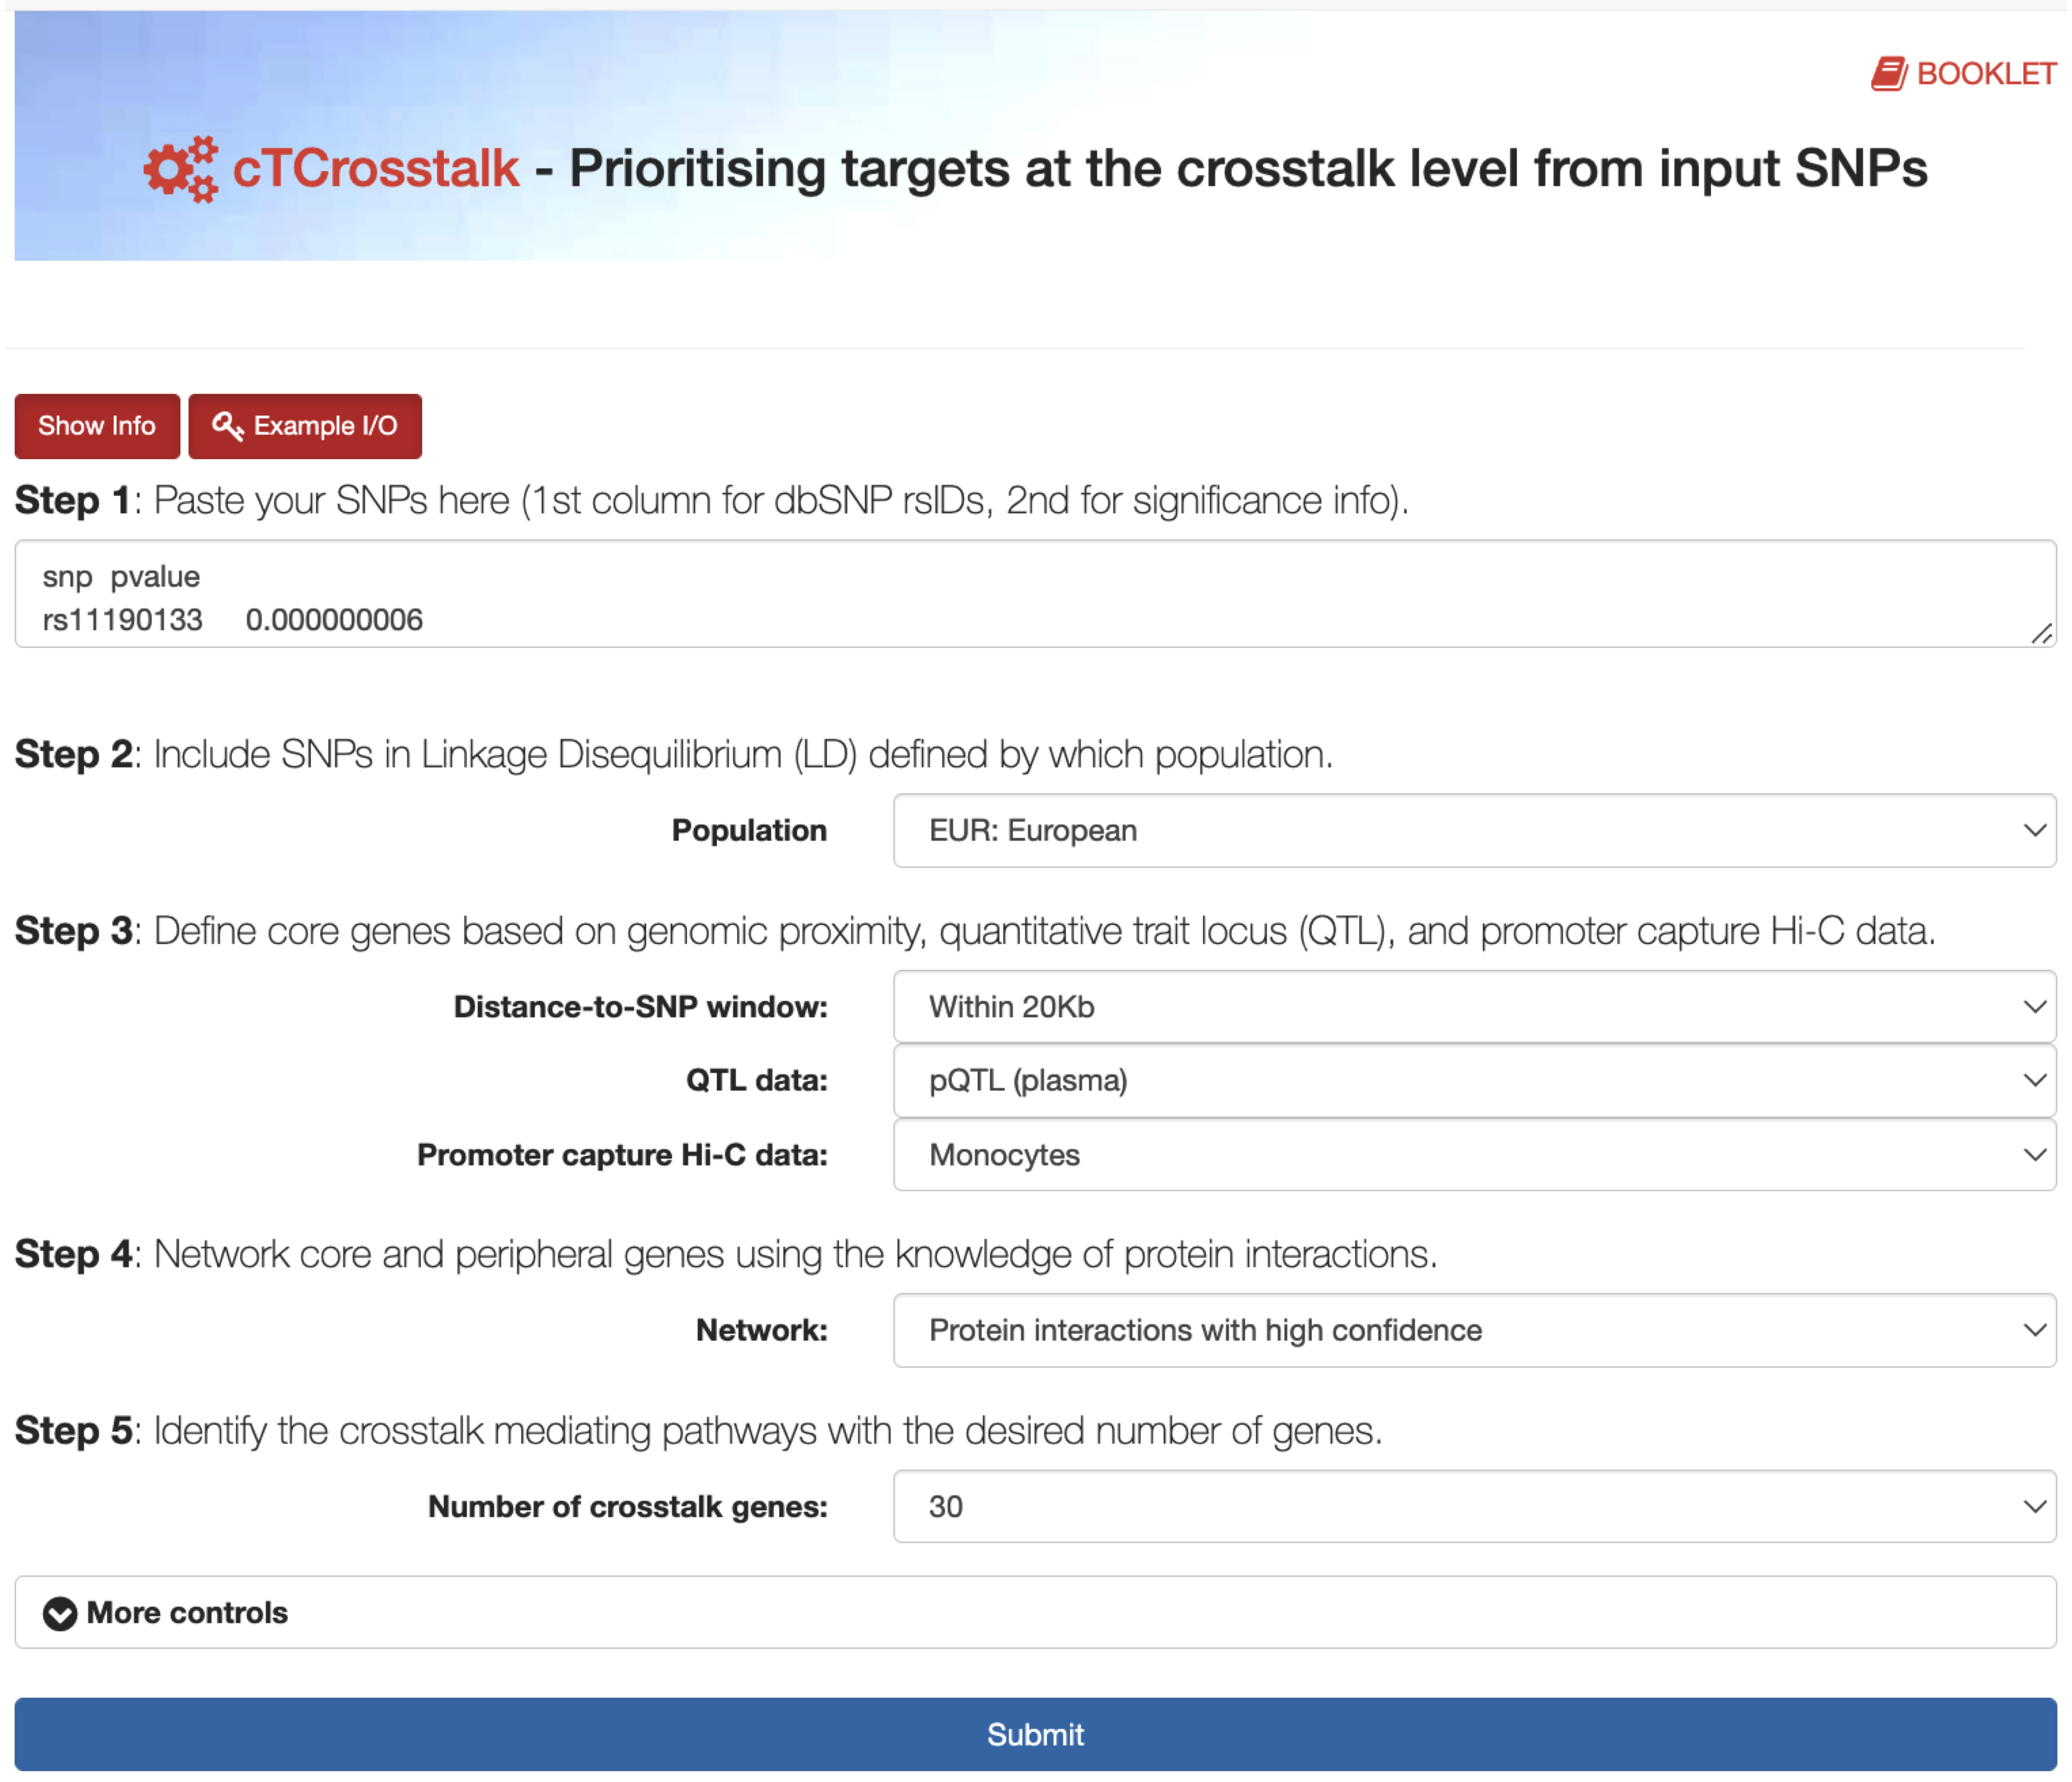
\includegraphics[width=1\linewidth]{index_files/figure-latex/cTCrosstalk-interface-1} 

}

\caption{The interface of cTCrosstalk, enabling/automating genetics-led and network-based identification and prioritisation of drug targets at the crosstalk level. The Show/Hide Info toggle button contains the help information on how to use cTCrosstalk, including input, output, mechanism, etc.}\label{fig:cTCrosstalk-interface}
\end{figure}

\hypertarget{prioritisation-results-1}{%
\section{Prioritisation results}\label{prioritisation-results-1}}

\begin{itemize}
\item
  \texttt{Output:\ target\ genes}: includes \texttt{Manhattan\ plot} illustrating priority rating for target genes that are color-coded by chromosomes. Also provided is the downloadable PDF file. It also includes \texttt{An\ interactive\ table} listing all prioritised genes, each receiving 5-star priority rating (scored 0-5). Genes are cross-referenced and linked out to GeneCards.
\item
  \texttt{Output:\ target\ pathways}: includes a dot plot and an interactive table for target pathways. Also provided is the downloadable PDF file.
\item
  \texttt{Output:\ targets\ at\ the\ crosstalk\ level}: includes \texttt{A\ network\ visualisation} illustrating the crosstalk between pathways, with genes colored by priority rating and labelled in the form of \texttt{rating@rank}, and \texttt{An\ interactive\ table}
  listing crosstalk genes, each receiving 5-star priority rating (scored 0-5). Genes are cross-referenced and linked out to GeneCards.
\item
  \texttt{Output:\ crosstalk-based\ drug\ repurposing}: includes \texttt{A\ heatmap-like\ illustration} showing drug repurposing analysis of approved drugs (licensed medications) based on pathway crosstalk genes, with crosstalk genes on y-axis, disease indications on x-axis, red dots indexed in number and referenced beneath in the table where the information on approved drugs and mechanisms of action is detailed. It also includes \texttt{An\ interactive\ table} of crosstalk genes (the column Crosstalk genes), disease indications (the column Disease indications), approved drugs and mechanisms (the column Approved drugs (mechanisms of action)), and drug index (the column Index) shown above within the dot plot.
\end{itemize}

\begin{figure}

{\centering 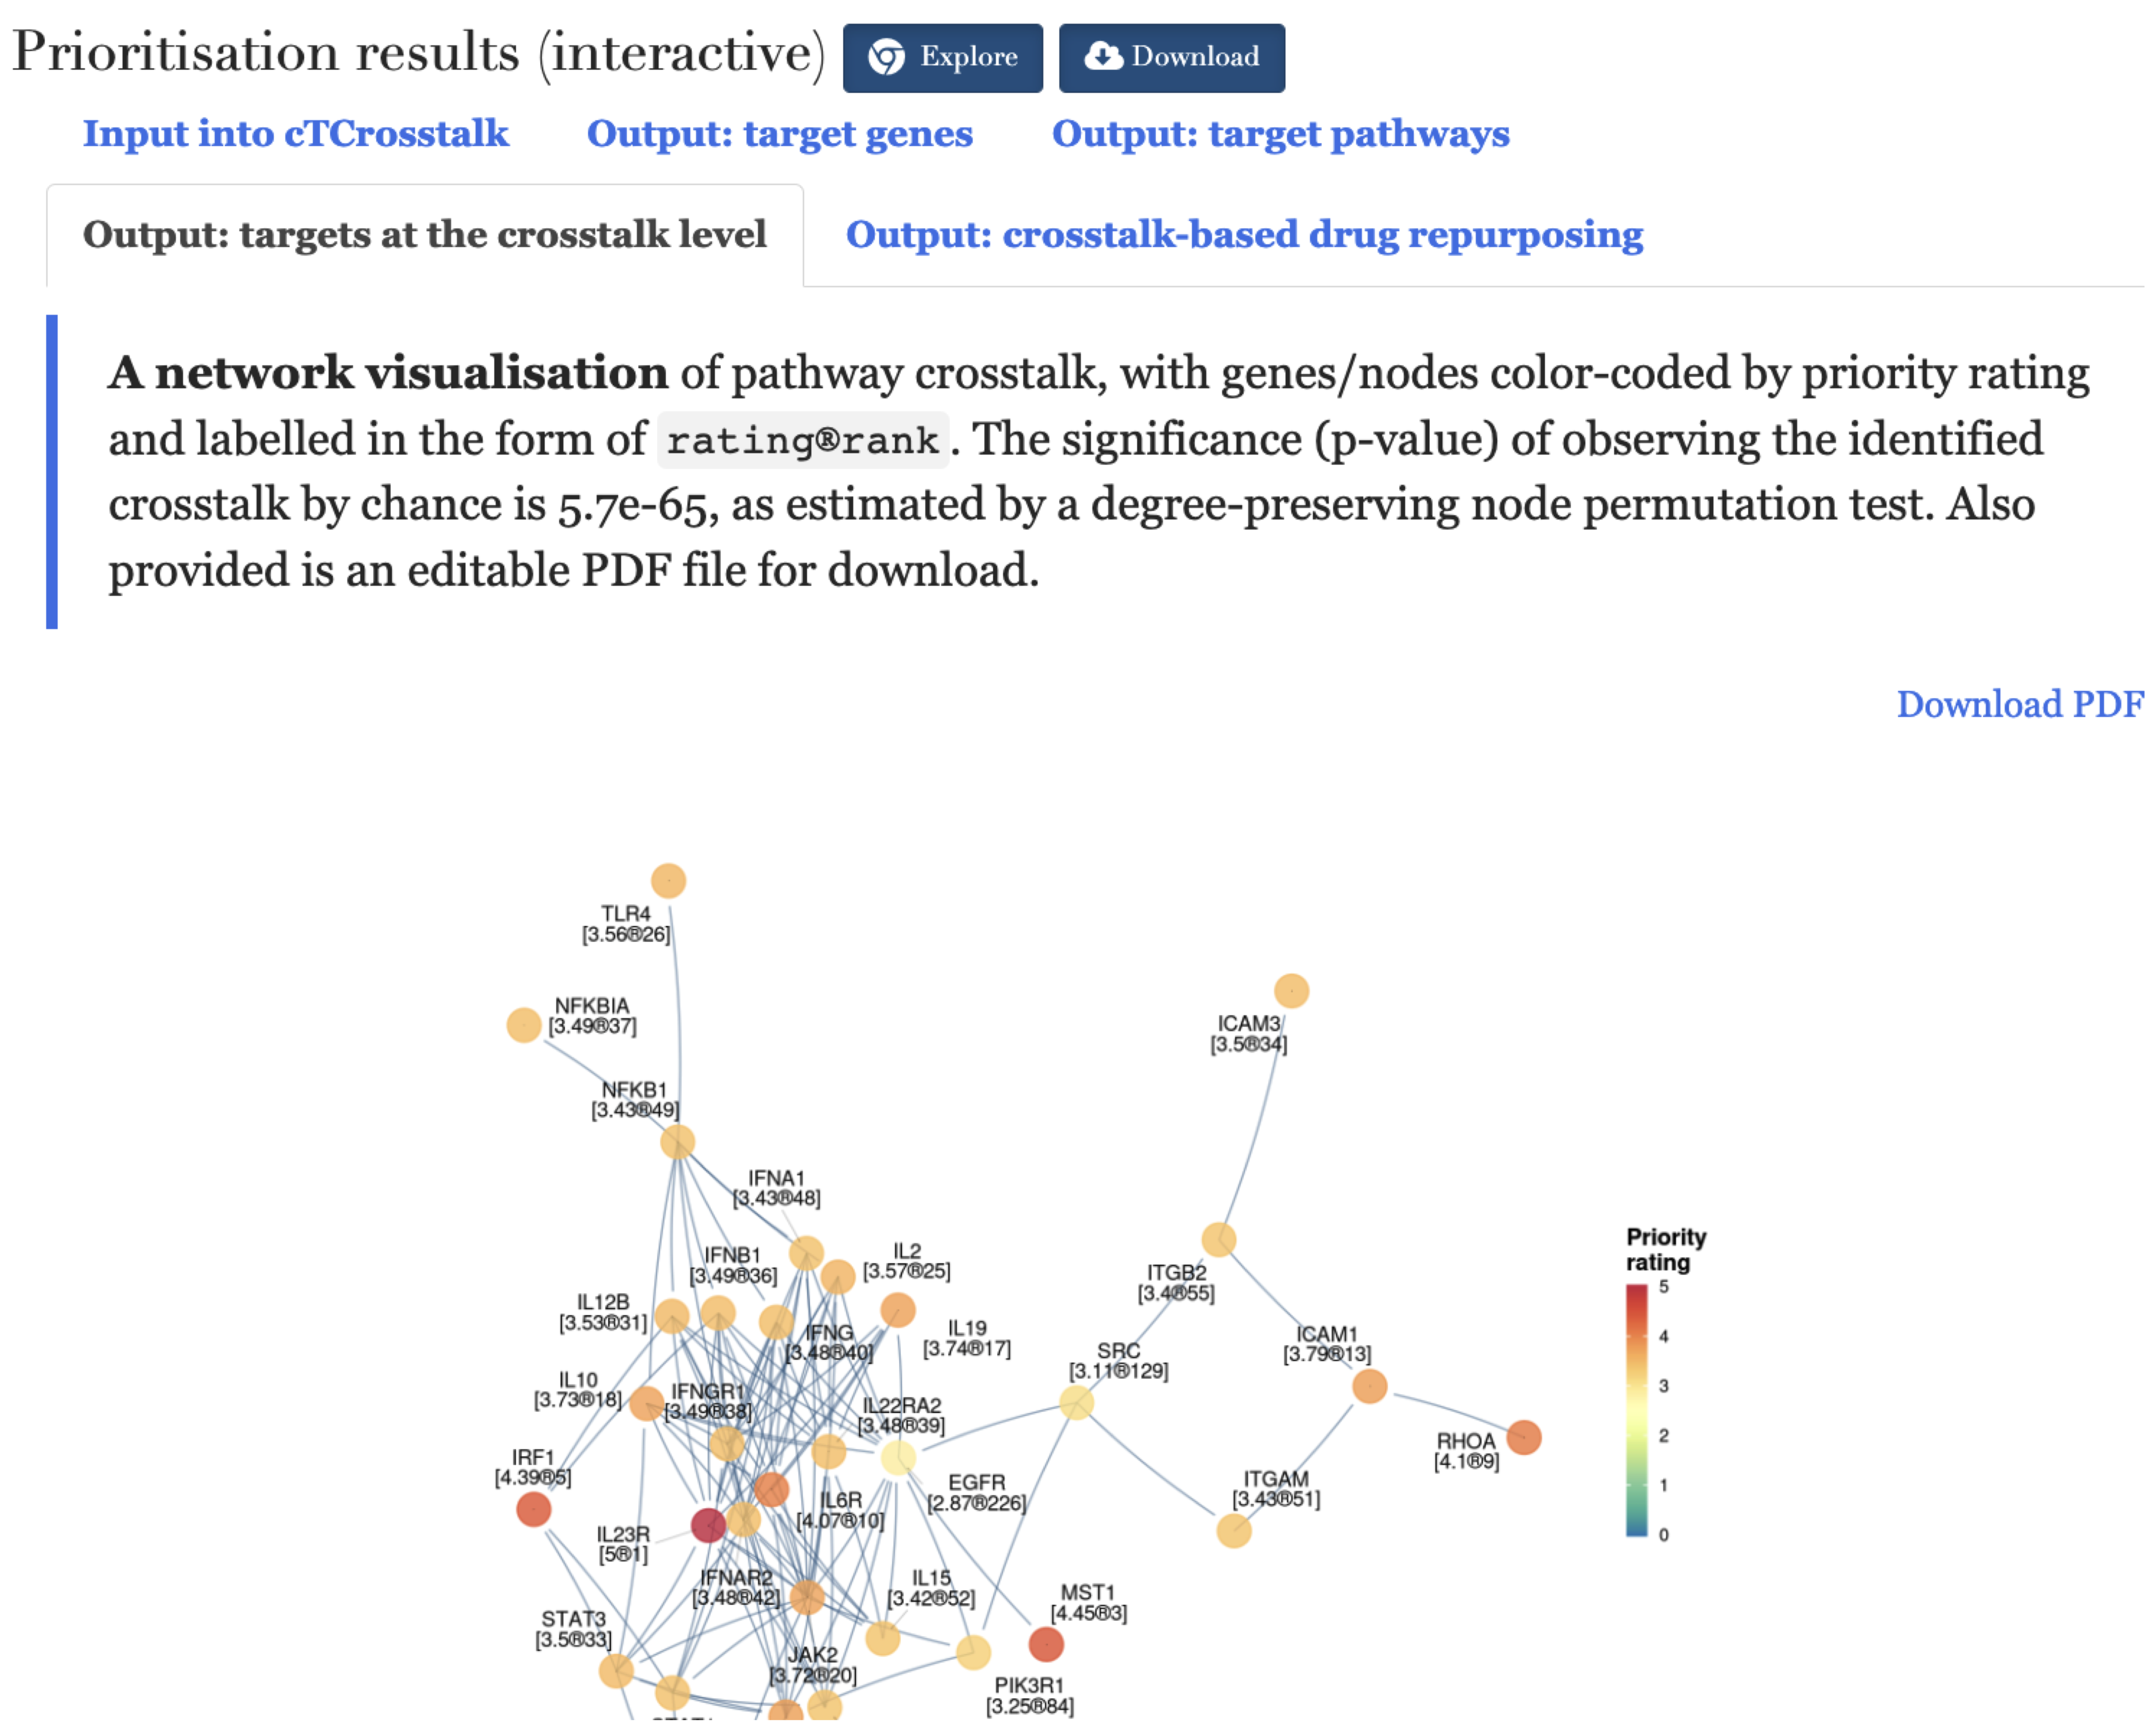
\includegraphics[width=1\linewidth]{index_files/figure-latex/cTCrosstalk-results-1} 

}

\caption{Interactive results for cTCrosstalk. The user input data are also returned for the exploration.}\label{fig:cTCrosstalk-results}
\end{figure}

\end{document}
